\documentclass[12pt]{extarticle}
\usepackage{geometry}
\geometry{
a4paper,
total={170mm,257mm},
left=20mm,
top=20mm,
headheight=12pt
}

\usepackage[parfill]{parskip} % Activate to begin paragraphs with an empty line rather than an indent
\usepackage{graphicx} % Use pdf, png, jpg, or eps§ with pdflatex; use eps in DVI mode
% TeX will automatically convert eps --> pdf in pdflatex
\graphicspath{ {./Figures/} }
\usepackage[labelfont=bf]{caption}
\usepackage{float}

\usepackage{amssymb,amsmath,amsthm}
\usepackage{commath}
\usepackage[hyphens]{url}
\usepackage[dvipsnames]{xcolor}
\usepackage[unicode=true,colorlinks=true,urlcolor=CadetBlue,citecolor=black,linkcolor=black]{hyperref}
\PassOptionsToPackage{hyphens}{url} % url is loaded by hyperref
\usepackage{authblk}
\usepackage{longtable}
\usepackage{multirow}
\usepackage{booktabs}
\usepackage{lipsum}  
\usepackage[title,page]{appendix}
\usepackage{chngcntr}
%\usepackage{endfloat}
      
%SetFonts
% newtxtext+newtxmath
\usepackage{newtxtext} %loads helv for ss, txtt for tt
\usepackage{amsmath}
\usepackage[bigdelims]{newtxmath}
\usepackage[T1]{fontenc}
\usepackage{textcomp}
%SetFonts

% less space before sections 
% \@startsection {NAME}{LEVEL}{INDENT}{BEFORESKIP}{AFTERSKIP}{STYLE} 
%            optional * [ALTHEADING]{HEADING} 
\makeatletter
 \renewcommand\section{\@startsection {section}{1}{\z@}%
     {-2.5ex \@plus -1ex \@minus -.2ex}%
     {1.3ex \@plus.2ex}%
    {\Large\bfseries}}
    
% Species names
%% Meta-Command for defining new species macros
\usepackage{xspace}

\newcommand{\species}[3]{%
  \newcommand{#1}{\gdef#1{\textit{#3}\xspace}\textit{#2}\xspace}}
  
\species{\yeast}{Saccharomyces cerevisiae}{S.~cerevisiae}
\species{\calbicans}{Candida albicans}{C.~albicans}
\species{\cneoformans}{Cryptococcus neoformans}{C.~neoformans}

% line numbers
\usepackage[displaymath, mathlines]{lineno}
\renewcommand\linenumberfont{\normalfont\small\sffamily}
\linenumbers
\modulolinenumbers[2]

% Yoav & Lee commands
\newcommand*{\tr}{^\intercal}
\let\vec\mathbf
\newcommand{\matrx}[1]{{\left[ \stackrel{}{#1}\right]}}
\newcommand{\diag}[1]{\mbox{diag}\matrx{#1}}
\newcommand{\goesto}{\rightarrow}
\newcommand{\dspfrac}[2]{\frac{\displaystyle #1}{\displaystyle #2} }
\newtheorem{theorem}{Theorem}
\newtheorem{corollary}{Corollary}
\newtheorem{lemma}{Lemma}
\newtheorem{remark}{Remark}
\newtheorem{result}{Result}
\renewcommand\qedsymbol{} % no square at end of proof
\newcommand{\cl}{\mathbf{L}}
\newcommand{\cj}{\mathbf{J}}
\newcommand{\ci}{I}

% Supplementary
% https://support.authorea.com/en-us/article/how-to-create-an-appendix-section-or-supplementary-information-1g25i5a/
\newcommand{\beginsupplement}{%
      	\setcounter{table}{0}
        \renewcommand{\thetable}{S\arabic{table}}%
        \setcounter{figure}{0}
        \renewcommand{\thefigure}{S\arabic{figure}}%
		\setcounter{equation}{0}
        \renewcommand{\theequation}{A\arabic{equation}}%
}

% autoref
\def\equationautorefname{Eq.}


% NatBib
\usepackage[round,colon]{natbib}

% Title page
\title{Non-Vertical Cultural Transmission, Assortment, \\and the Evolution of Cooperation}

% Authors
\renewcommand\Affilfont{\small}

\author[1]{Dor Cohen}
\author[2]{Ohad Lewin-Epstein}
\author[3]{Marcus W. Feldman}
\author[1,4,*]{Yoav Ram}

\affil[1]{School of Computer Science, Interdisciplinary Center Herzliya, Herzliya, Israel}
\affil[2]{School of Plant Sciences and Food Security, Tel Aviv University, Tel Aviv, Israel}
\affil[3]{Department of Biology, Stanford University, Stanford, CA}
\affil[4]{School of Zoology, Tel Aviv University, Tel Aviv, Israel}
\affil[*]{Corresponding author: yoav@yoavram.com}

\date{\today}

\begin{document}
\maketitle

% Abstract
\begin{abstract}
We study the cultural evolution of cooperation under vertical, horizontal, and oblique transmission.
Conditions are found for fixation and coexistence of cooperation and defection. 
We find that the evolution of cooperation is facilitated by horizontal transmission, especially when there is an association between cooperation and transmission, and that the effect of oblique transmission depends on the bias in horizontal transmission. Stable coexistence of cooperation and defection can occur. 
A spatial model is constructed and compared to results from an unstructured model.
Comparisons are drawn with Hamilton's rule and the concepts of relatedness and assortment.
% population mean fitness?
% TODO what about oblique?
\end{abstract}

\pagebreak


%%%%%%%%%%%%%%%%%%%%%%%%%%%
%%% Introduction
\section*{Introduction}
Cooperative behavior can reduce an individual's fitness and increase the fitness of its conspecifics or competitors~\citep{axelrod1981evolution}.
Nevertheless, cooperative behavior appears to occur in many non-human animals~\citep{dugatkin1997cooperation}, including primates~\citep{jaeggi2013natural},  rats~\citep{rice1962altruism}, birds~\citep{stacey1990cooperative,krams2008experimental}, and lizards~\citep{sinervo2006self}.
Evolution of cooperative behavior remains an important conundrum in evolutionary biology.

Since the work of  \citet{hamilton1964genetical} and \citet{axelrod1981evolution}, theories for the evolution of cooperative and altruistic behaviors have been intertwined often under the rubric of \emph{kin selection}.
Kin selection theory posits that natural selection is more likely to favor cooperation between more closely related individuals.
The importance of \emph{relatedness} to the evolution of cooperation and altruism was demonstrated by \citet{hamilton1964genetical}, who showed that an allele that determines cooperative behavior will increase in frequency if the reproductive cost to the actor that cooperates, $c$, is less than the benefit to the recipient, $b$, times the relatedness, $r$, between the recipient and the actor.
This condition is  known as \emph{Hamilton's rule}:
\begin{equation} \label{eq:hamilton_rule}
c < b \cdot r,
\end{equation}
where the relatedness coefficient $r$ measures the probability that an allele sampled from the cooperator is identical by descent to one at the same locus in the recipient.

\citet{Eshel1982} studied a related model for the evolution of cooperative behavior.
Their model included \emph{assortative meeting}, or non-random encounters, where a fraction $m$ of individuals in the population each interact with an individual of the same phenotype, and a fraction $1-m$ interacts  with a randomly chosen individual.  
Such assortative meeting may be due, for example, to population structure or active partner choice.
In their model, cooperative behavior can evolve if\footnote{In an extended model, which allows an individual to encounter $N$ individuals before choosing a partner, the righthand side is multiplied by $E[N]$, the expected number of encounters \citep[eq.~4.6]{Eshel1982}.
} 
\citep[eq.~3.2]{Eshel1982}
\begin{equation} \label{eq:eshel1982}
c < b \cdot m \,,
\end{equation}
where $b$ and $c$ are the benefit and cost of cooperation. 
Here $m$ in inequality~\ref{eq:eshel1982} takes the role of the relatedness coefficient $r$ in inequality~\ref{eq:hamilton_rule}.

The role of assortment in the evolution of altruism was emphasized by \citet{Fletcher2009assortment}.
They found that in a \emph{public-goods} game, altruism will evolve if cooperative individuals experience more cooperation, on average, than defecting individuals, and ``thus, the evolution of altruism requires (positive) assortment between focal \emph{cooperative} players and cooperative acts in their interaction environment.''
With some change in parameters, this condition is summarized by \citep[eq.~2.3]{Fletcher2009assortment}
\begin{equation} \label{eq:fletcher2009}
c < b \cdot (p_C - p_D ) \,,
\end{equation}
where $p_C$ is the probability that a cooperator receives help, and $p_D$ is the probability that a defector receives help.\footnote{Inequality~\ref{eq:fletcher2009} generalizes inequality~\ref{eq:hamilton_rule} and inequality~\ref{eq:eshel1982} by substituting $p_C=r + p$, $p_D=p$ and $p_C=m + (1-m)p$, $p_D=(1-m)p$, respectively, where $p$ is the frequency of cooperators.}
See \citet{Bijma2010assortment} for treatment of non-public-goods games.


In this paper we study the evolution of a cooperative behavior that is subject to \emph{cultural transmission}, which allows an individual to acquire attitudes or behavioral traits from other individuals in its social group through imitation, learning, or other modes of communication \citep{cavalli1981cultural,richerson2008not}.
\citet{feldman1985gene} introduced the first model for the evolution of altruism by cultural transmission.
They demonstrated that if the fidelity of cultural transmission of altruism is $\varphi$, then the condition for evolution of altruism in the case of sib-to-sib altruism is \citep[Eq.~16]{feldman1985gene}
\begin{equation} \label{eq:feldman1985}
c < b \cdot \varphi - \frac{1-\varphi}{\varphi} \,.
\end{equation}
In inequality~\ref{eq:feldman1985}, $\varphi$ takes the role of relatedness ($r$ in inequality~\ref{eq:hamilton_rule}) or assortment ($m$ in inequality~\ref{eq:eshel1982}), but the effective benefit $b\cdot \varphi$ is  reduced by $(1-\varphi)/\varphi$. This shows that under a combination of genetic and cultural transmission, the condition for the evolutionary success of altruism entails a modification of Hamilton's rule (\ref{eq:hamilton_rule}).

Cultural transmission may be  viewed as vertical, horizontal or oblique:  vertical transmission occurs between parents and offspring, horizontal transmission occurs between individuals from the same generation, and oblique transmission occurs  to offspring from the generation to which their parents belong (i.e. from non-parental adults). 
Evolution under either of these transmission models can be be more rapid than under pure vertical transmission~\citep{cavalli1981cultural,lycett2008questions,ram2018evolution}.
Both \citet{woodcock2006significance} and \citet{lewin2017microbes} demonstrated that non-vertical transmission can help explain the evolution of cooperative behavior (the former using simulations with cultural transmission, the latter using a model where cooperation is mediated by microbes that manipulate their host's behavior.) 
Some of the analyses by \citet{lewin2017microbes} can be applied to cultural transmission, because models of cultural transmission are mathematically similar to those for transmission of infectious diseases~\citep{cavalli1981cultural}.

Here, we study cultural-evolution models of cooperation that include both vertical and non-vertical transmission. 
We investigate these models using mathematical analysis and simulations.  
In our models behavioral changes are mediated by cultural transmission that can occur specifically during social interactions.
For instance, there may be an association between the choice of partner for social interaction and the choice of partner for cultural transmission.
As another example, when an individual interacts with an individual of a different phenotype,  exposure to the latter may lead the former to  convert its phenotype.
Our results demonstrate that cultural transmission can enhance the evolution of cooperation even when genetic transmission cannot, partly because it facilitates the generation of assortment \citep{Fletcher2009assortment}, and partly because non-vertical transmission can protect traits from the effect of natural selection \citep{ram2018evolution}.
This further emphasizes that treatment of cooperation as a cultural trait, rather than a genetic one, can lead to a broader understanding of its evolutionary dynamics.


%%%%%%%%%%%%%%%%%%%%%%%%%%%
% Models
\section*{Models}

Consider a large population whose members can be one of two phenotypes: $\phi=A$ for cooperators or $\phi=B$ for defectors.
An offspring inherits its phenotype from its parent via vertical transmission with probability $v$ or from a random individual in the parental population via oblique transmission with probability $(1-v)$. 
Following~\citet{ram2018evolution}, given that the parent phenotype is $\phi$ and assuming uni-parental inheritance, % TODO cite Zefferman Behav Ecol 2016
the conditional probability that the phenotype $\phi'$ of the offspring is $A$ is 

\begin{equation} \label{eq:vertical_oblique_transmission}
P(\phi'=A \mid \phi) = \begin{cases}
v + (1-v)p, & \text{if } \phi=A \\
(1-v)p, & \text{if } \phi=B
\end{cases},
\end{equation}
where $p=P(\phi=A)$ is the frequency of $A$ among all adults in the parental generation.  

Not all adults become parents due to natural selection, and we denote the frequency of phenotype $A$ among parents by $\tilde{p}$.
Therefore, the frequency $\hat{p}$ of  phenotype $A$ among juveniles (after selection and vertical and oblique transmission) is

\begin{equation}\label{eq:horizontal}
\begin{aligned}
\hat{p}
& = \tilde{p} [v + (1-v)p] + (1-\tilde{p}) [(1-v)p] \\
& = v \tilde{p} + (1-v) p \;.
\end{aligned}
\end{equation}

Individuals are assumed to interact according to a \emph{prisoner's dilemma}.
Specifically, individuals interact in pairs; a cooperator suffers a fitness cost $0<c<1$, and its partner gains a fitness benefit $b$, where we assume $c<b$. \autoref{table:prisoner_payoff} shows the payoff matrix, i.e. the fitness of an individual with phenotype $\phi_1$ when interacting with a partner of phenotype $\phi_2$.

%%% Table: payoff matrix
\bigskip
\begin{table}[h]
\centering
\caption{\textbf{Payoff matrix for prisoner's dilemma.}
The fitness of phenotype $\phi_1$ when interacting with phenotype $\phi_2$. $A$ is a cooperative phenotype, $B$ is a defector phenotype, $b$ is the benefit gained by an individual interacting with a cooperator, and $c$ is the cost of cooperation. $b>c>0$.
}
\begin{tabular}{lll}
\toprule
           & $\phi_2=A$ & $\phi_2=B$ \\ \cmidrule(r){1-3}
$\phi_1=A$ & $1+b-c$ & $1-c$ \\
$\phi_1=B$ & $1+b$   & $1$
\\ \bottomrule
\end{tabular}
\label{table:prisoner_payoff}
\end{table}
\bigskip
%%%


Social interactions occur randomly:
two juvenile individuals with phenotype $A$ interact with probability $\hat{p}^2$, two juveniles with phenotype $B$ interact with probability $(1-\hat{p})^2$, and two juveniles with different phenotypes interact with probability $2\hat{p}(1-\hat{p})$. 

Horizontal cultural transmission occurs between pairs of individuals from the same generation. 
It occurs between socially interacting partners with probability $\alpha$, or between a random pair with probability $1-\alpha$ (see~\autoref{fig:horizontal}).
%The social association $\alpha$ is therefore the fraction of population that receives (horizontal transmission) from the social interaction partner, and $1-\alpha$ receives randomly.
However, horizontal transmission is not always successful, as one partner may reject the other's phenotype. The probability for successful horizontal transmission of phenotypes $A$ and $B$ are $T_A$ and $T_B$, respectively (\autoref{table:interactions}).

%%% Table: interactions
\bigskip
\begin{table}[]
\caption{\textbf{Interaction frequency, fitness, and transmission probabilities.}}
\begin{tabular}{@{}llllll@{}}
\toprule
\multirow{2}{*}{Phenotype $\phi_1$} &
  \multirow{2}{*}{Phenotype $\phi_2$} &
  \multirow{2}{*}{Frequency} &
  \multirow{2}{*}{Fitness of $\phi_1$} &
  \multicolumn{2}{l}{$P(\phi_1=A)$ via horizontal transmission:} \\ \cmidrule(l){5-6} 
    &     &                      &         & from partner, $\alpha$ & from population, $(1-\alpha)$ \\ \cmidrule(r){1-6}
$A$ & $A$ & $\hat{p}^2$          & $1+b-c$ & 1                      & $\hat{p}+(1-\hat{p})(1-T_B)$  \\
$A$ & $B$ & $\hat{p}(1-\hat{p})$ & $1-c$   & $1-T_B$                & $\hat{p}+(1-\hat{p})(1-T_B)$  \\
$B$ & $A$ & $\hat{p}(1-\hat{p})$ & $1+b$   & $T_A$                  & $\hat{p} T_A$                 \\
$B$ & $B$ & $(1-\hat{p})^2$      & $1$     & $0$                    & $\hat{p} T_A$                 \\ \bottomrule
\end{tabular}
\label{table:interactions}
\end{table}
\bigskip
%%%


Therefore, the frequency $p'$ of phenotype $A$ among adults in the next generation, after horizontal transmission, is 
\begin{equation}\label{eq:nextgen_adults}
\begin{aligned}
p'
& = \hat{p}^2 [\alpha + (1-\alpha)(\hat{p} + (1-\hat{p})(1-T_B))] \\
& + \hat{p}(1-\hat{p}) [\alpha(1-T_B) + (1-\alpha)(\hat{p} + (1-\hat{p})(1-T_B))] \\
& + (1-\hat{p})\hat{p} [\alpha T_A + (1-\alpha) \hat{p} T_A ] \\
& + (1-\hat{p})^2 [(1-\alpha) \hat{p} T_A] \;,
\end{aligned}
\end{equation}
which simplifies to
\begin{equation}\label{eq:nextgen_adults_slimpify}
p' = \hat{p}^2(T_B-T_A) + \hat{p}(1+T_A-T_B) .
\end{equation}

The frequency of $A$ among parents (i.e. after selection) follows a similar dynamic, but also includes the effect of natural selection, and is therefore
\begin{equation}\label{eq:nextgen_parents}
\begin{aligned}
\bar{w} \tilde{p}'
& = \hat{p}^2 (1+b-c) [\alpha + (1-\alpha)(\hat{p} + (1-\hat{p})(1-T_B))] \\
& + \hat{p}(1-\hat{p}) (1-c) [\alpha(1-T_B) + (1-\alpha)(\hat{p} + (1-\hat{p})(1-T_B))] \\
& + (1-\hat{p})\hat{p} (1+b) [\alpha T_A + (1-\alpha) \hat{p} T_A ] \\
& + (1-\hat{p})^2 [(1-\alpha) \hat{p} T_A] \;,
\end{aligned}
\end{equation}
where fitness values are taken from \autoref{table:prisoner_payoff} and \autoref{table:interactions}, and the population mean fitness is
\begin{equation} \label{eq:mean_fitness}
\bar{w} =  1 + \hat{p}(b-c).
\end{equation}

\autoref{eq:nextgen_parents} can be simplified to
\begin{equation}\label{eq:nextgen_parents_simplified}
\begin{aligned}
\bar{w} \tilde{p}'
& = \hat{p}^2 (1+b-c) \big(1-(1-\hat{p})(1-\alpha)T_B)\big) \\
& + \hat{p}(1-\hat{p}) (1-c) \big(\hat{p}(1-\alpha)T_B+1-T_B\big) \\
& + (1-\hat{p})\hat{p} (1+b) \big(\hat{p}(1-\alpha) + \alpha\big) T_A \\
& + (1-\hat{p})^2 \hat{p} (1-\alpha) T_A \;.
\end{aligned}
\end{equation}
%where $\hat{p}=v\tilde{p}+(1-v)p$.
\autoref{table:vars_params} summarizes the model variables and parameters.

%%% Table: variables and parameters
\bigskip
\begin{table}[h]
\centering
\caption{\textbf{Model variables and parameters.}
}
\begin{tabular}{lll}
\toprule
Symbol & Description & Values \\ \cmidrule(r){1-3}
$A$ & Cooperator phenotype & \\
$B$ & Defector phenotype & \\
$p$ & Frequency of phenotype $A$ among adults & $[0,1]$ \\
$\tilde p$ & Frequency of phenotype $A$ among parents & $[0,1]$ \\
$\hat p$ & Frequency of phenotype $A$ among juveniles & $[0,1]$ \\
$v$ & Vertical transmission rate & $[0,1]$ \\
$c$ & Cost of cooperation & $(0,1)$ \\
$b$ & Benefit of cooperation & $c<b$ \\
$\alpha$ & Probability of social association & $[0,1]$ \\
$T_A, T_B$ & Horizontal transmission rates of phenotype $A$ and $B$ & $[0,1]$ \\
\\ \bottomrule
\end{tabular}
\label{table:vars_params}
\end{table}
%\bigskip
%%%


%%%%%%%%%%%%%%%%%%%%%%%%%%%
%%% Results
\section*{Results}


%%%%%%%%%%%%%%%%%%%%%%%%%%%%%%%%%%%%%%%%%%%%%%%%
\subsection*{Oblique and Horizontal Transmission}

With only oblique and horizontal transmission, i.e. $v = 0$, Eq.\ \ref{eq:horizontal} becomes $\hat{p}=p$ and Eq.\ \ref{eq:nextgen_adults_slimpify} becomes % TODO check this, I changed the ref from nextgen_parents_simplified to nextgen_adults_slimpify
\begin{equation}  \label{eq:nextgen_parents_oblique_only}
p' = p^2 (T_B-T_A) + p (1+T_A-T_B) \;,
\end{equation}

which gives the following result.\\

\begin{result}[Oblique and horizontal transmission of cooperation] \label{result:obli_hori}
Without vertical transmission ($v=0$), if there is a horizontal transmission bias in favor of cooperation, namely
\begin{equation} \label{eq:oblique_only_result}
T_A > T_B \;,
\end{equation}
then the frequency of the cooperator phenotype among adults increases every generation, $p'>p$.
\end{result}

That is, in the absence of vertical transmission, selection plays no role in the evolution of cooperation (i.e. $b$ and $c$ are missing from \autoref{eq:nextgen_parents_oblique_only}).
The dynamics are determined solely by differential horizontal transmission of the two phenotypes, namely, the relative tendency of each phenotype to be horizontally transmitted to peers (see~{\autoref{fig:results}c).
Note that without bias in horizontal transmission, $T_A = T_B$, phenotype frequencies are static, $p'=p$.


%%%%%%%%%%%%%%%%%%%%%%%%%%%%%%%%%%%%%%%%%%
\subsection*{Vertical and Horizontal Transmission}

With only vertical and horizontal transmission, i.e. $v=1$, Eq.\ \ref{eq:horizontal} becomes
$\hat{p} =  \tilde{p}$,
and Eq.\ \ref{eq:nextgen_parents_simplified} for the frequency of the cooperative phenotype among parents in the next generation $\tilde{p}'$ can be written as
\begin{equation} \label{eq:nextgen_parents_vertical_only} 
\begin{aligned}
\bar{w} \tilde{p}' 
& = \tilde{p}^2 (1+b-c) [1 - (1-\tilde{p}) (1-\alpha) T_B] \\
& + \tilde{p}(1-\tilde{p}) (1-c) [\tilde{p} (1-\alpha) T_B + 1 - T_B] \\
& + \tilde{p}(1-\tilde{p}) (1+b) [\tilde{p} (1-\alpha) + \alpha] T_A \\
& + (1-\tilde{p})^2 \tilde{p} (1-\alpha) T_A \;.
\end{aligned}
\end{equation}

Fixation of either cooperation, $\tilde{p}=1$, or defection, 
$\tilde{p}=0$, are equilibria of Eq.\ \ref{eq:nextgen_parents_vertical_only}, solving $\tilde{p}'= \tilde{p}$.
We assume for the remainder of the analysis that $0<\tilde{p}<1$.

If $\alpha=1$, then $\tilde{p}'= \tilde{p}$ reduces to
\begin{equation}
\tilde{p}(1-\tilde{p})\big[(1+b)T_A + (1-c)(1-T_B)-1\big] = 0 \;,
\end{equation}
and there are no additional equilibria.
For cooperation to take over the population (i.e., for $\tilde{p}=1$ to be globally stable) we require $\tilde{p}'>\tilde{p}$; that is,
\begin{equation}
  \tilde{p}^2 (1+b-c) + \tilde{p}(1-\tilde{p}) \big[(1-c) (1 - T_B) + (1+b)T_A\big] 
  > \bar{w}\tilde{p} \;.
\end{equation}
Factoring out $\tilde{p}(1-\tilde{p})$ and setting $\bar{w} = 1 + \tilde{p}(b-c)$, we find that $\hat{p}'>\hat{p}$ if
%\begin{equation}
%  (1-\tilde{p}) \big[(1-c) (1 - T_B) + (1+b)T_A\big] 
%  > 1 -\tilde{p} .
%\end{equation}
%Dividing by $(1-\tilde{p})$ we find that $\tilde{p}'>\tilde{p}$ if 
\begin{equation} \label{eq:vert_hori_alpha1_condition_proof}
  (1-c) (1 - T_B) + (1+b)T_A > 1 \;.
\end{equation}
\\

If $\alpha<1$, divide both sides of Eq.\ \ref{eq:nextgen_parents_vertical_only} by $\tilde{p}$ and set $\bar{w} = 1 + \tilde{p}(b-c)$. Then $\tilde{p}'>\tilde{p}$ if
\begin{equation}
\begin{aligned} 
  1 + \tilde{p}(b-c) < 
  & \, \tilde{p}(1+b-c) (1 - (1-\tilde{p}) (1-\alpha) T_B) \\
  & + (1-\tilde{p}) (1-c) (\tilde{p} (1-\alpha) T_B + 1 - T_B) \\
  & + (1-\tilde{p}) (1+b) (\tilde{p} (1-\alpha) + \alpha) T_A \\
  & + (1-\tilde{p})^2 (1-\alpha) T_A \;.
\end{aligned}
\end{equation}
%Rearranging, we get
%\begin{equation} 
%\begin{aligned} 
%  1 - \tilde{p} < 
%  & - \tilde{p}(1+b-c)(1-\tilde{p}) (1-\alpha) T_B \\
%  & + (1-\tilde{p}) (1-c) (\tilde{p} (1-\alpha) T_B + 1 - T_B) \\
%  & + (1-\tilde{p}) (1+b) (\tilde{p} (1-\alpha) + \alpha) T_A \\
%  & + (1-\tilde{p})^2 (1-\alpha) T_A .
%\end{aligned}
%\end{equation}
%Diving by $(1-\tilde{p})$ and rearranging so that free terms are on the left and terms with $\tilde{p}$ are on the right, we have
%\begin{equation} 
%\begin{aligned} 
%  &1 - (1-\alpha) T_A - (1+b) \alpha T_A - (1 - T_B)(1-c)  < \\
%   &\tilde{p}[ - (1+b-c) (1-\alpha) T_B 
%   + (1-c) (1-\alpha) T_B
%   + (1+b) (1-\alpha) T_A 
%   - (1-\alpha) T_A].
%\end{aligned}
%\end{equation}
Simplifying, we find that $\tilde{p}'>\tilde{p}$ if and only if
\begin{equation} \label{eq:vert_hori_global_condition}
c(1-T_B) - b \alpha T_A - (T_A-T_B) < \tilde{p} \cdot b (1-\alpha) (T_A-T_B) \;.
\end{equation}

In addition to the the fixation states $\tilde{p}=0$ and $\tilde{p}=1$, there may be an actual polymorphic equilibrium of $\tilde{p}'=\tilde{p}$ in Eq.\ \ref{eq:nextgen_parents_vertical_only}, namely 
\begin{equation} \label{eq:vert_hori_equilibrium}
  \tilde{p}^* = 
  \frac{c(1-T_B) - b \alpha T_A - (T_A-T_B)}{b (1-\alpha) (T_A-T_B)} ,
\end{equation} 
which is legitimate if $0<\tilde{p}^*<1$.

Since all parameters are positive, we can apply
inequality \ref{eq:vert_hori_global_condition} and see that a requirement for $\tilde{p}'>\tilde{p}$ is that either 
\begin{align} 
\label{eq:vert_hori_global_condition1}
T_A > T_B \quad&\text{and}\quad \tilde{p}>\tilde{p}^*,  \quad \text{or} \\
\label{eq:vert_hori_global_condition2}
T_A <T_B \quad&\text{and}\quad \tilde{p}<\tilde{p}^* .
\end{align}

We define the \emph{cost boundaries},
\begin{equation} \label{eq:cost_boundaries}
\begin{aligned}
\gamma_1 = \frac{b \alpha T_A + (T_A - T_B)}{1-T_B}, \quad
\gamma_2 = \frac{b \alpha T_B + (1+b) (T_A - T_B)}{1-T_B}.
\end{aligned}
\end{equation}
Then, applying Eqs.~\ref{eq:vert_hori_equilibrium}, \ref{eq:vert_hori_global_condition1}, and \ref{eq:vert_hori_global_condition2}, we  summarize the possible outcomes in the following result and corollaries.
\\

\begin{result}[Vertical and horizontal transmission of cooperation] \label{result:vert_hori}
With vertical and horizontal but without oblique transmission ($v=1$), the cultural evolution of cooperation exhibits one of the following scenarios, depending on the cost boundaries $\gamma_1$ and $\gamma_2$ (\autoref{eq:cost_boundaries}):

%\begin{enumerate} % p* version
%\item Fixation of cooperation,
%	if $T_A>T_B$ and $0<\tilde{p}^*$, or
%	if $T_A>T_B$ and $0<\tilde{p}^*<1$, and $\tilde{p}_0>\tilde{p}^*$, or
%	if $T_A<T_B$ and $1<\tilde{p}^*$.
%\item Global fixation of defection,
%	if $T_A>T_B$ and $\tilde{p}^*>1$, or
%	if $T_A>T_B$ and $0<\tilde{p}^*<1$, and $\tilde{p}_0<\tilde{p}^*$, or
%	if $T_A<T_B$ and $\tilde{p}^*<0$
%\item Co-existence of both phenotypes at $\tilde{p}^*$, 
%	if $T_A<T_B$ and $0<\tilde{p}^*<1$.
%\end{enumerate}
\begin{enumerate} % gamma version
\item \emph{Fixation of cooperation}:
	if \emph{(i)} $T_A \ge T_B$ and $c < \gamma_1$; or
	if \emph{(ii)} $T_A < T_B$ and $c < \gamma_2$.
\item \emph{Fixation of defection}:
	if \emph{(iii)} $T_A \ge T_B$ and $\gamma_2 < c$; or
	if \emph{(iv)} $T_A < T_B$ and $\gamma_1 < c$.
\item \emph{Stable coexistence}:
	if \emph{(v)} $T_A<T_B$ and $\gamma_2 < c < \gamma_1$.
\item \emph{Unstable coexistence}: 
	if \emph{(vi)} $T_A>T_B$ and $\gamma_1 < c <\gamma_2$.
\end{enumerate}
\end{result}

These conditions are illustrated in \autoref{fig:results2}.

Cooperation and defection can coexist stably at frequencies $\tilde{p}^*$ and $1-\tilde{p}^*$ (\autoref{eq:vert_hori_equilibrium}) if there is horizontal transmission bias for defection, $T_A<T_B$, and the cost of cooperation is intermediate, $\gamma_2 < c < \gamma_1$; see yellow area in \autoref{fig:results2}b.
When unstable coexistence occurs, phenotype $A$ will fix if its initial frequency is $p>\tilde{p}^*$, and phenotype $B$ will fix if its initial frequency is $1-p>1-\tilde{p}^*$; this occurs when there is horizontal transmission bias for cooperation, $T_A>T_B$, and the cost is intermediate, $\gamma_1 < c < \gamma_2$.
\autoref{fig:coexistence_without_oblique} shows the mapping $\tilde p \to \tilde p'$; see blue areas in \autoref{fig:results2}a and \autoref{fig:results2}b.
\\

\begin{corollary}[Symmetric horizontal transmission] \label{sec:sym_hor_trans}
If $T=T_A=T_B$, then cooperation will take over the population if
\begin{equation}
\label{eq:equal_transmission}
c < b \cdot \alpha \frac{T}{1-T} \;.
\end{equation}
\end{corollary}
Note that the right-hand side equals $\gamma_1$ when $T=T_A=T_B$.
This condition is obtained by setting $T=T_A=T_B$ in inequality \ref{eq:vert_hori_global_condition} and can be interpreted as a version of Hamilton's rule  ($c<b\cdot r$, inequality~\ref{eq:hamilton_rule}) or as a version of inequality~\ref{eq:fletcher2009}, where $\alpha T/(1-T)$ can be regarded as the \emph{effective relatedness} or \emph{effective assortment}, respectively.
\autoref{fig:results}a illustrates this condition. 

The condition in inequality~\ref{eq:equal_transmission} demonstrates the importance of the social association $\alpha$. The following corollaries provide additional demonstrations.
\\

\begin{corollary}[Perfect social association of transmission and cooperation]
With perfect social association ($\alpha=1$), the only equilibria are the fixation states, $\tilde{p}=0$ and $\tilde{p}=1$, and cooperation will evolve from any initial frequency (i.e., $\tilde{p}'>\tilde{p}$) if
\begin{equation}\label{eq:vert_hori_alpha1}
c < \frac{b \cdot T_A + (T_A - T_B)}{1-T_B}.
\end{equation}
\end{corollary}
This condition is obtained from inequality \ref{eq:vert_hori_alpha1_condition_proof}, and the right-hand side equals $\gamma_1$ when $\alpha=1$ (\autoref{eq:cost_boundaries}).
Perfect social association (horizontal transmission always occurs during the cooperative interaction) is also assumed in the model studied by \citet{lewin2017microbes}, and therefore this corollary is equivalent to the result in their eq.~1.

%In terms of the cost boundaries, inequality~\ref{eq:vert_hori_alpha1} is equivalent to $c<\gamma_1$, and if $T_A>T_B$ then that suffices for fixation of cooperation. If $T_B>T_A$ then $\gamma_2(\alpha=1)<0$ and again, inequality~\ref{eq:vert_hori_alpha1} is sufficient for increase in the frequency of $A$.
Inequality~\ref{eq:vert_hori_alpha1} can also be written as
$1 - (1-c)(1-T_B) < (1+b) T_A$,
which provides an interesting interpretation for the success of cooperation. 
In the interaction between a cooperator and a defector, $(1-c)(1-T_B)$ is the probability that the cooperator remains cooperative and also reproduces. 
Therefore, $1 - (1-c)(1-T_B)$ is the probability that either the cooperator becomes a defector, or that it fails to reproduce.
This is the \emph{effective cost of cooperation} from this interaction.
Similarly, $(1+b) T_A$ is the probability that during an interaction between a cooperator and a defector, the defector becomes cooperative and reproduces, which is the \emph{effective benefit of cooperation} from this interaction.
Thus, inequality~\ref{eq:vert_hori_alpha1} entails that cooperation can evolve if the effective cost of cooperation is less than the effective benefit during an interaction between a cooperator and a defector.
\\

\begin{corollary}[No social association of transmission and cooperation]
Without social association ($\alpha=0$), cooperation can take over the population if there is horizontal transmission bias for cooperation, $T_A>T_B$, and if either
\begin{equation}
\label{eq:vert_hori_alpha0}
c < \frac{T_A-T_B}{1-T_B}
\quad \text{or} \quad
\tilde{p}_0 > \tilde{p}^* = \frac{c(1-T_B) - (T_A-T_B)}{b (T_A-T_B)} \;.
\end{equation}
\end{corollary}

\autoref{fig:results2}a illustrates these conditions, which are obtained by setting $\alpha=0$ in Eqs.\ \ref{eq:vert_hori_equilibrium} and \ref{eq:cost_boundaries}. If there is horizontal transmission bias for cooperation ($T_A>T_B$) then cooperation can evolve from any initial frequency if the cost is low enough, $c<\gamma_1$ (green area below solid line). If the cost is not low enough, cooperation can also evolve if its initial frequency is high enough and the cost is not too high, $c<\gamma_2$ (blue area between solid and dashed lines). 

We can interpret these condition as follows. First, when cooperators are rare, they will mostly interact with defectors. Therefore, for cooperation to increase in frequency and fix, the \emph{effective cost of cooperation} must be lower than the horizontal transmission of cooperation, $1-(1-c)(1-T_B) < T_A$, which is equivalent to the first of the two inequalities in \autoref{eq:vert_hori_alpha0}.
Second, if $T_A$ is not large enough, cooperation will fix if the initial frequency is higher than the threshold $\tilde{p}^*$; thus, this threshold must be below one, which entails $1-(1-c)(1-T_B) < T_A + b(T_A-T_B)$. That is, the effective cost of cooperation must be lower than the combined effect of horizontal transmission of cooperation, $T_A$, and the benefit of cooperation multiplied by the transmission bias, $b(T_A-T_B)$. 
\\

Given the previous two corollaries for no association and perfect association ($\alpha=0$ and $\alpha=1$), it is interesting to examine the general effect of social association on the evolution of cooperation.
We denote the social association boundaries by
\begin{equation}\begin{aligned}\label{eq:boundries_assortative_meeting}
  a_1 = \frac{c(1-T_B)-(1+b)(T_A-T_B)}{b\cdot T_B}, \quad
  a_2 = \frac{c(1-T_B)-(T_A-T_B)}{b\cdot T_A}.
\end{aligned}\end{equation}
Applying Eqs.~\ref{eq:vert_hori_equilibrium}, \ref{eq:vert_hori_global_condition1}, and \ref{eq:vert_hori_global_condition2}, we have the following corollary.
\\

\begin{corollary}[Intermediate association of transmission and cooperation]\label{corollary:Intermediate_association}
Cooperation will increase from rarity if social association is high enough, specifically if
  \begin{equation} \label{eq:unequal_transmission_from_rarity_in_alpha_terms}
    \begin{aligned}
    T_A > T_B &\;\; \text{and} \;\; a_2 < \alpha, \quad \text{or} \\
    T_A < T_B &\;\; \text{and} \;\; a_1 < \alpha \,.
    \end{aligned}
    \end{equation} 
\end{corollary}

\autoref{fig:results2}c demonstrates these conditions.
With horizontal transmission bias for cooperation ($T_A>T_B$), cooperation can fix from any initial frequency if $a_2<\alpha$ (green area in positive x-axis). 
Otherwise, cooperation can also fix if the horizontal bias is strong, the initial frequency is high, and social association is high, $a_1 < \alpha$ (blue area).
With horizontal bias favoring defection ($T_A<T_B$), cooperation can fix from any frequency if social association is high, $a_1<\alpha$ (green area with $T_A<T_B$), and can also increase when rare and reach stable coexistence with defection if social association is intermediate, $a_2<\alpha$ (yellow area).
Without horizontal bias ($T_A=T_B$) fixation of cooperation occurs if social association is high enough; $\frac{c}{b} \cdot \frac{1-T}{T} < \alpha$ (inequality~\ref{eq:equal_transmission}; in this case $a_1=a_2$).



%%%%%%%%%%%%%%%%%%%%%%%%%%%%%%%%%%%%%%%%%%%%%%%%
\subsection*{With Vertical and Oblique Transmission}

With both vertical and oblique transmission, $0<v<1$, the recursion system is more complex
and we focus on local rather than on global stability.
To proceed,  note that 
Eq.\ \ref{eq:horizontal} gives $\hat{p}'$ as a function of both $p'$ and $\tilde{p}'$.
%Equation 4 does not give $\hat{p}$---MF
Eq.\ \ref{eq:nextgen_adults_slimpify} gives $p'$ as a function of $\tilde{p}$, since $\hat{p}$ is given in Eq.\ \ref{eq:horizontal} as a function of $\tilde{p}$ and 
Eq.\ \ref{eq:nextgen_parents_simplified} gives $\tilde{p}'$ as a function of $\hat{p}$. 
Combining these equations, we find an equation for $\hat{p}'$ as a function of $\hat{p}$ (shown in Appendix~\autoref{sec:appendixA}),
determine the equilibria, namely, solutions of $\hat{p}' = \hat{p}$, and analyse their local stability.
%: an equilibrium $\hat{p}^*$ is locally stable when the derivative of $f(\hat{p})=\bar{w}(\hat{p}'-\hat{p})$ at the equilibrium is negative, $f'(\hat{p}^*)<0$. 

%We start with the simple case of symmetrical horizontal transmission, $T=T_A=T_B$ and apply \autoref{eq:horizontal}, \autoref{eq:nextgen_adults_slimpify}, and \autoref{eq:nextgen_parents_simplified} to obtain 
%\begin{equation} \label{eq:equal_horizontal_transmission}
%\begin{aligned}
%  f(\hat{p}) &= 
%  \bar{w}(\hat{p}' - \hat{p}) = \\
%  &\hat{p}(1-\hat{p})\big[\alpha bvT - cv(1-T)\big].\end{aligned}
%\end{equation}
%A detailed explain of how we get eq.~\ref{eq:equal_horizontal_transmission} can be found in appendix B.
%The equilibria are solutions of $f(\hat{p})=0$, or $\hat{p}' = \hat{p}$.
%It is easy to verify that fixation of either phenotype, $\hat{p} =  0$ and $\hat{p} = 1$, is an equilibrium.
%Since the derivative of $f'(\hat{p}$ is 
%\begin{equation}
%f'(\hat{p})=(1-2\hat{p})\big[\alpha bvT - cv(1-T)\big],
%\end{equation}
%then the condition for local stability of $\hat{p}=1$ is
%\begin{equation} \label{eq:derivative_of_phattag-phat}
%	f'(1) =	-\alpha bvT + cv(1-T) < 0,
%\end{equation}
%which gives the following result.
%
%\textbf{Result 3: Oblique and vertical transmission with symmetric horizontal transmission.}
%If horizontal transmission is symmetric, $T = T_A = T_B$, and if
%\begin{equation} \label{eq:oblique_and_vertic_result2}
%  %\frac{b}{c}>\frac{1-T}{\alpha T}
%	c < b \cdot \frac{\alpha T}{1-T},
%\end{equation}
%then fixation of the cooperator phenotype $A$ is locally stable.
%The same condition was given in Corollary 1.1, \autoref{eq:equal_transmission}.

%We now turn to the general case where $T_A \neq T_B$. 
Applying Eqs.\ \ref{eq:horizontal}, \ref{eq:nextgen_adults_slimpify}, and \ref{eq:nextgen_parents_simplified} gives the function $f(\hat{p})$ (see Appendix~\autoref{sec:appendixA}):

\begin{equation} \label{eq:general_case_polynomial}
  f(\hat{p}) = \bar{w}(\hat{p}'-\hat{p}) =
  \beta_1 \hat{p}^3 + \beta_2 \hat{p}^2 + \beta_3 \hat{p},
\end{equation}
where 
\begin{equation} \label{eq:polynomial_coefficients}
\begin{aligned}
\beta_1 &= \big[c(1-v) - b (1-\alpha v)\big] (T_A-T_B) , \\
\beta_2 &= -\beta_1 -\beta_3 ,  \\
\beta_3 &= \alpha bvT_A - cv(1-T_B) + (T_A-T_B) .
\end{aligned}
\end{equation}

If $T=T_A=T_B$ then $\beta_1=0$ and $\beta_3=-\beta_2=\alpha b vT -cv(1-T)$, 
and $f(\hat{p})$ becomes a quadratic polynomial:
\begin{equation} \label{eq:equal_horizontal_transmission}
  f(\hat{p}) = \hat{p}(1-\hat{p})\big[\alpha bvT - cv(1-T)\big].
\end{equation}
Clearly the only two equilibria are the fixations  $\hat{p} =  0$ and $\hat{p} = 1$.
These equilibria are locally stable if $f'(\hat{p})<0$ near the equilibrium (see Appendix~\autoref{sec:appendixB}), where
\begin{equation}
f'(\hat{p})=(1-2\hat{p})\big[\alpha bvT - cv(1-T)\big],
\end{equation}
with
\begin{equation} \label{eq:derivative_of_phattag-phat}
\begin{aligned}
	f'(0) &=	\alpha bvT - cv(1-T), \\
	f'(1) &=	-\alpha bvT + cv(1-T).
\end{aligned}
\end{equation}
Therefore with symmetric horizontal transmission ($T_A=T_B$), fixation of the cooperative phenotype ($\hat{p}=1$) occurs under the same condition as Corollary 1.1, namely Eq.\ \ref{eq:equal_transmission}.


In the general case where $T_A \neq T_B$, the coefficient $\beta_1$ is not necessarily zero, and $f(\hat{p})$ is a cubic polynomial.
Therefore, three equilibria may exist, two of which are
$\hat{p} = 0 $ and $\hat{p} = 1$, and the third is
\begin{equation} \label{eq:oblique_and_vertic_result}
  \hat{p}^* =  
  \frac{\beta_3}{\beta_1}.
\end{equation}

Note that the sign of the  cubic (Eq.\ \ref{eq:general_case_polynomial}) at positive (negative) infinity is equal (opposite) to the sign of $\beta_1$. 
If $T_A>T_B$, then 
\begin{equation} \label{eq:beta1}
   \beta_1 < [c(1-\alpha v) - b(1-\alpha v)] (T_A-T_B) 
   = (1-\alpha v)(c-b)(T_A-T_B) < 0 ,
 \end{equation}
since $c<b$ and $\alpha v < 1$. Hence the signs of the cubic at positive and negative infinity are negative and positive, respectively.
First, if $\beta_3<\beta_1$ then 
$1<\hat{p}^*$ and therefore $f'(0)<0$ and $f'(1)>0$; that is, fixation of the defector phenotype $B$ is the only locally stable legitimate (i.e. between 0 and 1) equilibrium.
Second, if $\beta_1<\beta_3<0$ then 
$0<\hat{p}^*<1$ and therefore $f'(0)<0$ and $f'(1)<0$ so that both fixations are locally stable and $\hat{p}^*$ separates the domains of attraction.
Third, if $0<\beta_3$ then 
$\hat{p}^*<0$ and therefore $f'(0)>0$ and $f'(1)<0$; that is, fixation of the cooperator phenotype $A$ is the only locally stable legitimate equilibrium.

Similarly, if $T_A<T_B$, then
\begin{equation} \label{eq:beta1_rev}
   \beta_1 > [c(1-\alpha v) - b(1-\alpha v)] (T_A-T_B) 
   = (1-\alpha v)(c-b)(T_A-T_B) > 0,
 \end{equation}
since $c<b$ and $\alpha v < 1$, and the signs of the cubic at positive and negative infinity are positive and negative, respectively. 
First, if $\beta_3<0$ then $\hat{p}^*<0$ and therefore $f'(0)<0$ and $f'(1)>0$; that is, fixation of the defector phenotype $A$ is the only locally stable legitimate equilibrium.
Second, if $0<\beta_3<\beta_1$ then $0<\hat{p}^*<1$ and therefore $f'(0)>0$ and $f'(1)>0$; that is, both fixations are locally unstable and $\hat{p}^*$ is a stable polymorphic equilibrium.
Third, if $\beta_1<\beta_3$ then $\hat{p}^*>1$ and therefore $f'(0)>0$ and $f'(1)<0$, and fixation of the cooperator phenotype $A$ is the only locally stable legitimate equilibrium.

Define new cost boundaries, $\hat\gamma_1$ and $\hat\gamma_2$,
\begin{equation} \label{eq:cost_boundaries_v}
\begin{aligned}
\hat\gamma_1 = \frac{b v \alpha T_A + (T_A - T_B)}{v(1-T_B)}, \quad
\hat\gamma_2 = \frac{b v \alpha T_B + (1+b) (T_A - T_B)}{v(1-T_B) + (1-v)(T_A-T_B)},
\end{aligned}
\end{equation}
and  a vertical transmission threshold,
\begin{equation} \label{eq:v_threshold}
\hat v = \frac{T_B - T_A}{1-T_A} \,.
\end{equation}

Now, assume $T_A<T_B$.
$\beta_3<0$ requires $\hat\gamma_1<c$,
and for $\beta_3<\beta_1$ we need $c\big[v(1-T_B) + (1-v)(T_A-T_B)\big] > bv\alpha T_B + (1+b)(T_A-T_B)$.
Note that the expression in the square brackets is positive if and only if $v > \hat v$.
Thus, for $\beta_3<\beta_1$ we need $v > \hat v$ and $\hat\gamma_2 < c$ or $v < \hat v$ and $c < \hat\gamma_2$,
and for $0<\beta_3<\beta_1$ we need $v > \hat v$ and $\hat\gamma_2 < c < \hat\gamma_1$, or $v < \hat v$ and $c < \min(\hat\gamma_1, \hat\gamma_2)$. For $\beta_1<\beta_3$ we need $v > \hat v$ and $c<\hat\gamma_2$ or $v < \hat v$ and $\hat\gamma_2<c$.
However, some of these conditions cannot be met, since $v < \hat v$ implies $c<1<\hat\gamma_2$.
A similar analysis can be made when $T_A>T_B$.

The following result summarizes the possible outcomes.
\\

\begin{result}[Vertical, oblique, and horizontal transmission of cooperation] \label{result:vert_obli_hori}
With vertical, horizontal, and oblique transmission, the cultural evolution of a cooperator phenotype will follow one of the following scenarios depending on the cost boundaries $\hat\gamma_1$ and $\hat\gamma_2$ (\autoref{eq:cost_boundaries_v}) and the vertical transmission threshold $\hat v$ (\autoref{eq:v_threshold}) :

% in beta
%\begin{enumerate}
%\item \emph{Fixation of cooperation}: 
%	if \emph{(i)} $T=T_A=T_B$ and $c < b\cdot \frac{\alpha T}{1-T}$; or
%	if \emph{(ii)} $T_A>T_B$ and $0<\beta_3$; or 
%	if \emph{(iii)} $T_A<T_B$ and $\beta_1<\beta_3$.
%\item \emph{Fixation of the defection}: 
%	if \emph{(iv)}  $T=T_A=T_B$ and $c > b\cdot \frac{\alpha T}{1-T}$; or 
%	if \emph{(v)} $T_A>T_B$ and $\beta_3<\beta_1<0$; or 
%	if \emph{(vi)} $T_A<T_B$ and $\beta_3<0$.
%\item \emph{Coexistence of both phenotypes at $\hat{p}^*$}: 
%	if \emph{(vii)} $T_A < T_B$ and $0<\beta_3<\beta_1$.
%\item \emph{Fixation of either phenotype depending on initial frequency}:
%	if \emph{(viii)}  $T_A>T_B$ and $\beta_1<\beta_3<0$.
%\end{enumerate}

% in gamma
\begin{enumerate}
\item \emph{Fixation of cooperation}: 
	if \emph{(i)} $T_A \ge T_B$ and $c < \hat\gamma_1$; or 
	if \emph{(ii)} $T_A < T_B$ and $v>\hat v$ and $c < \hat\gamma_2$.
\item \emph{Fixation of defection}: 
    if \emph{(iii)} $T_A \ge T_B$ and $\hat\gamma_2 < c$; or 
	if \emph{(iv)} $T_A < T_B$ and $\hat\gamma_1 < c$.
\item \emph{Stable Coexistence}: 
    if \emph{(v)} $T_A < T_B$ and $v>\hat{v}$ and $\hat\gamma_2 < c < \hat\gamma_1$; or
    if \emph{(vi)} $T_A < T_B$ and $v<\hat{v}$ and $c < \hat\gamma_1$.
\item \emph{Unstable coexistence}:
    if \emph{(vii)} $T_A > T_B$ and $\hat\gamma_1 < c < \hat\gamma_2$.
\end{enumerate}

\end{result}
These conditions are illustrated in \autoref{fig:result3}ab.

Much of the literature on evolution of cooperation focuses on conditions for  initially rare cooperative phenotype to invade a population of defectors.
The next corollary deals with such a condition.
\\

\begin{corollary}[Condition for cooperation to increase from rarity]
  If the initial frequency of cooperation is very close to zero, $\hat{p}_0 \approx 0$, then its frequency will increase if 
  \begin{equation} \label{eq:unequal_transmission_from_rarity_general_case}
  \begin{aligned}
  c < \hat\gamma_1 = \frac{b v \alpha T_A + (T_A - T_B)}{v(1-T_B)} \;.
  \end{aligned}
  \end{equation} 
  \end{corollary}

%Note that the right-hand side equals $\hat\gamma_1$.
This condition merges the conditions for fixation of cooperation and for stable coexistence, which both lead to the instability of $\hat{p}=0$, the fixation of defection.
Importantly, increasing social association $\alpha$ increases maximum cost of cooperation $\hat\gamma_1$ that allows cooperation to increase from rarity (i.e. $\partial \hat\gamma_1 / \partial \alpha > 0$).

In general, this condition cannot be formulated in the form of Hamilton's rule due to the horizontal transmission bias $T_A-T_B$.
Without horizontal transmission bias, i.e., with $T=T_A=T_B$, these conditions reduce to a form of Hamilton's rule.
\\
\begin{corollary}[Necessary condition for fixation of cooperation]
  Fixation of cooperation is possible only if the vertical transmission rate is high enough,
  \begin{equation} \label{eq:fixation_of_cooperation_vertical_transmission_condition}
    \begin{aligned}
      v>\hat{v} = \frac{T_B - T_A}{1-T_A} \;.
    \end{aligned}
    \end{equation} 
\end{corollary}
%Note that $\sigma \frac{\partial \gamma_1}{\partial v} = \sigma (T_B-T_A)$ and $\sigma \frac{\partial \hat\gamma_2}{\partial v} = \sigma (T_A-T_B)(b \alpha T_B - (1+b)(1-T_A))$
Note that this condition does not guarantee fixation of cooperation. Rather, if this condition does not apply then cooperation cannot fix.
When horizontal transmission is biased for cooperation, $T_A>T_B$, cooperation can fix with any vertical transmission rate, i.e. $\hat{v}<0$.
In contrast, if the horizontal transmission is biased for defection, $T_A<T_B$,  cooperation can fix only if the vertical transmission rate is high enough: in this case oblique transmission can prevent fixation of cooperation, see \autoref{fig:result3}bd.
\\

In corollary~\autoref{corollary:Intermediate_association}, we examined the effect of social association on evolution of cooperation in the case of perfect vertical transmission ($v=1$).
A more general case can be stated for $0 < v \leq 1$.
Consider the social association boundaries 
\begin{equation}\begin{aligned}\label{eq:boundries_assortative_meeting_general_case}
  \hat{a}_1 = \frac{c\cdot v(1-T_A) -(T_A-T_B)(1+b-c)}{b\cdot v \cdot T_B}, \quad
  \hat{a}_2 = \frac{c\cdot v(1-T_B)-(T_A-T_B)}{b\cdot v\cdot T_A} \;.
\end{aligned}\end{equation}
Then the following applies.
\\

\begin{corollary}[Intermediate association of transmission and cooperation]\label{corollary:Intermediate_association}
Cooperation will increase from rarity if social association is high enough, specifically if
  \begin{equation} \label{eq:unequal_transmission_from_rarity_in_alpha_terms}
    \begin{aligned}
    T_A > T_B &\;\; \text{and} \;\; \hat a_2 < \alpha, \quad \text{or} \\
    T_A < T_B &\;\; \text{and} \;\; \hat a_1 < \alpha \,.
    \end{aligned}
    \end{equation} 
\end{corollary}
\autoref{fig:result3}cd illustrates this conditions.

Interestingly, when $T_A>T_B$ then $\partial \hat a_2 / \partial v = b T_A (T_A-T_B) > 0$, and when $T_A<T_B$ then $\partial \hat a_1 / \partial v = b(1+b-c)T_B(T_A-T_B) < 0$.
Therefore, when there is horizontal transmission bias for cooperation, $T_A>T_B$, then vertical transmission hinders the evolution of cooperation ($\partial \hat a_2 / \partial v = b T_A (T_A-T_B) > 0$). In contrast, when there is horizontal transmission bias for defection, vertical transmission facilitates the evolution of cooperation ($\partial \hat a_1 / \partial v = b(1+b-c)T_B(T_A-T_B) < 0$).



%%%%%%%%%%%%%%%%%%%%%%%%%%%%%%%%%%%%%%%%%%%%%%%%
\subsection*{With population structure}

Social association may also emerge from a population's structure.
Consider a  population colonizing a 2D grid of size 100-by-100, where each site is inhabited by one individual, similarly to \citet{lewin2020rockpaperscissors}.
Each individual is characterized by its phenotype which is either cooperator, $A$, or defector $B$.
In each generation individuals interact with their neighbors, i.e. individuals that inhabit adjacent sites, in a prisoner's dilemma game (\autoref{table:prisoner_payoff}) and with horizontal cultural transmission.
As before, $T_A$ and $T_B$ are the probabilities of transmitting phenotypes $A$ and $B$ during horizontal transmission.
At each generation, each individual is chosen to "initiate" interactions with probability 1/2.\ %"with probability 1/2" not clear - MWF
Initiators then interact with a random neighbor in a prisoners' dilemma game and a random neighbor (with replacement) for horizontal cultural transmission (as both the game and the transmission are symmetrical, the expected number of each of these interactions per individual per generation is 1).
Therefore, the effective social association $\alpha$ in this model is the probability that the same neighbor is picked for both interactions, or $\alpha=1/m$, where $m$ is the number of neighbors. On an infinite grid, $m=8$, but on a finite grid $m$ can be lower in edge neighborhoods close to the grid border.
%How are A, B initialized on the grid? – MWF

The order of the interactions across the lattice at each generation is random.
After all interactions take place, and individual's fitness is determined by
$w = 1 + b \cdot n_b - c \cdot n_c$,
where $n_b$ is the number interactions of that individual with cooperative neighbors, and $n_c$ is the total number of interactions that that individual  had ($n_b \le n_c$).
Then a new generation is generated.
Each site is colonized by an offspring of one of the individuals that inhabit either this site or one of the neighboring sites.
The parent is randomly drawn with probability proportional to its fitness, divided by the average fitness in its neighborhood.
Offspring then have the same phenotype as their parents.

\autoref{fig:spatial} shows that the highest cooperation cost to benefit ratio ($c/b$) that permits the evolution of cooperation in simulations of the spatial model is roughly $\alpha \cdot T / (1-T)$, where $T=T_A=T_B$ is the horizontal transmission rate. This agrees with the condition we derived in Corollary~\ref{sec:sym_hor_trans} for a population without population structure, and 
this demonstrates that the social association parameter $\alpha$ can emerge from local interactions between individuals in a structured population.


%%%%%%%%%%%%%%%%%%%%%%%%%%%
% Discussion
\section*{Discussion}
We studied the evolution of cooperation under non-vertical transmission using deterministic discrete-time evolutionary models with fitnesses in the form of payoffs from a prisoner's dilemma game. 
Under oblique and horizontal cultural transmission, horizontal transmission bias in favor of the cooperative phenotype was found to be necessary and sufficient for evolution of cooperation (Result~\autoref{result:obli_hori}).
Under a combination of vertical, oblique, and horizontal transmission, cooperation or defection can either fix or coexist at a stable polymorphism, depending on the relationship between the cost and benefit of cooperation, the horizontal bias, and the association between cooperation and transmission (Results~\autoref{result:vert_hori} and~\autoref{result:vert_obli_hori}).
Remarkably, stable coexistence between cooperation and defection can be maintained if horizontal transmission is biased for defection ($T_A<T_B$) and both the cost of cooperation and social association are intermediate (yellow areas in \autoref{fig:results2}).
% TODO figure for result 3
% TODO something about v-hat

We tested the applicability of our analytic results. Our derived analytic condition provided a good approximation to simulation results for a complex spatial stochastic model  (\autoref{fig:spatial}), demonstrating that association between cooperation and transmission can arise in a structured population simply because the choice of individuals for social interactions is very restricted.

\citet{feldman1985gene} studied the dynamics of an altruistic phenotype with vertical cultural transmission and a gene that modifies the transmission of the phenotype. Their results are very sensitive to this genetic modification: without it, the conditions for invasion of the altruistic phenotype reduce to Hamilton's rule.
Further work is needed to incorporate such genetic modification of cultural transmission into our model.

\citet{woodcock2006significance} stressed the significance of non-vertical transmission for the evolution of cooperation. He executed simulations with prisoner's dilemma payoffs but without horizontal transmission or social association ($\alpha=0$). Nevertheless, his results demonstrated that it is possible to sustain altruistic behavior via cultural transmission for a substantial length of time.
Our results provide strong evidence for his hypothesis that horizontal transmission can have an important role in the evolution of cooperation. 

To understand the role of horizontal transmission, we first discuss the role of \emph{assortment}.
\citet{Eshel1982} showed that altruism can evolve when there is enough \emph{assortative meeting}, namely, a tendency for individuals to interact within their phenotypic group.
\citet{Fletcher2009assortment}  further argued that a general explanation for the evolution of altruism is given by \emph{assortment}: the correlation between individuals that carry an altruistic trait and the amount of altruistic behavior in their interaction group (see also \citet{Bijma2010assortment}).
They therefore suggested that to explain the evolution of altruism, we should seek mechanisms that generate  assortment, such as population structure, repeated interactions, and individual recognition.
Our results highlight another mechanism for generating assortment: an association between social interactions and horizontal transmission that creates a correlation between one's partner for interaction and partner for transmission.
This mechanism does not require population structure, repeated interactions, or individual recognition.
We show that high levels of such social association greatly increase the potential for evolution of cooperation (\autoref{fig:results2}).
With enough social association ($\alpha > \big(c(1-T_B) + (T_B-T_A)\big) / b T_A$), cooperation can increase in frequency when initially rare even when there is horizontal transmission bias against it ($T_A<T_B$, see Result~\autoref{result:vert_hori}).

How does non-vertical transmission generate assortment? 
\citet{lewin2017microbes} and \citet{lewin2020rockpaperscissors} 
suggested that microbes that manipulate their hosts to act altruistically can be favored by selection, which may help to explain the evolution of cooperation. 
%Indeed, it has been shown that microbes can mediate behavioral changes in their  hosts~\citep{dobson1988population,poulin2010parasite}. 
%Therefore, natural selection on microbes may favor manipulation of the host so that it cooperates with others. 
From the kin selection point-of-view, if microbes can be transmitted \emph{horizontally} from one host to another during host interactions, then following horizontal transmission the recipient host will carry microbes that are closely related to those of the donor host, 
even when the two hosts are (genetically) unrelated. 
From the assortment point-of-view,
infection by behavior-determining microbes during interactions effectively generates assortment because a recipient of help may be infected by a behavior-determining microbe and consequently become a helper.
Cultural horizontal transmission can similarly generate assortment between the cooperative phenotype and the benefit of cooperation if cultural transmission and helping interactions occur between the same individuals, which in our model occurs with probability $\alpha$. 

Thus, with horizontal transmission, ``assortment between focal cooperative players and cooperative acts in their interaction
environment''~\citep{Fletcher2009assortment} is generated not because \emph{the helper is likely to be helped}, but rather because \emph{the helped is likely to become a helper}.
These conclusions highlight the importance of non-vertical cultural transmission in explaining complex evolutionary phenomena, and  furthers our understating of the cultural evolution of cooperation. 

% Javarone MA, Atzeni AE, Galam S. Emergence of Cooperation in the Prisoner ’ s Dilemma Driven by Conformity. 2:155-163. doi:10.1007/978-3-319-16549-3


%%%%%%%%%%%%%%%%%%%%%%%%%%%
% \pagebreak
% Acknowledgements
{\small
\section*{Acknowledgements}
We thank Lilach Hadany and Ayelet Shavit for discussions and comments.
This work was supported in part by
the Israel Science Foundation 552/19 (YR),
and Minerva Stiftung Center for Lab Evolution (YR).
% TODO funding for other authors?
}



%%%%%%%%%%%%%%%%%%%%%%%%%%%
% Appendices
\begin{appendices}
\renewcommand{\theequation}{\thesection\arabic{equation}}
\counterwithin*{equation}{section}

%%%%%%%%%%%%%%%%%%%%%%%%%%%%%%%%%%%%%%%%%%%%%%%%%%%%%
\section{} \label{sec:appendixA}
We want to find the frequency of juveniles with phenotype $A$ in next generation $\hat{p}'$ as a function of frequency
of juveniles with phenotype $A$ in the current generation $\hat{p}$.
Starting from \autoref{eq:horizontal},
\begin{equation}\label{eq:appendix_b_1}
  \hat{p}' = v \tilde{p}' + (1-v) p',
\end{equation}
 substitute for $p'$ using \autoref{eq:nextgen_adults_slimpify} and for $\tilde{p}'$ using \autoref{eq:nextgen_parents_simplified}, we have
\begin{equation}\label{eq:appendix_b_2}
  \begin{aligned}
  \hat{p}'  = & \frac{v}{\bar{w}}\left\{\hat{p}^2(1+b-c)\left[1-(1-\hat{p})(1-\alpha)T_B)\right]\right\} \\
  & + \frac{v}{\bar{w}}\left\{ \hat{p}(1-\hat{p})(1-c)\left[ \hat{p}(1-\alpha)T_B + 1 - T_B \right] \right\} \\
  & + \frac{v}{\bar{w}}\left\{ \hat{p}(1-\hat{p})(1+b)\left[\hat{p}(1-\alpha) + \alpha \right]T_A \right\} \\
  & + \frac{v}{\bar{w}}(1-\hat{p})^2\hat{p}(1-\alpha)T_A \\
  & + (1-v)\hat{p}^2(T_B-T_A) + (1-v)\hat{p}(1+T_A-T_B),
\end{aligned}
\end{equation}
where $\bar{w} = 1 + \hat{p}(b-c)$. 
Define $g(\hat{p})$ as
\begin{equation} \label{eq:appendix_define_f}
\begin{aligned}
      g(\hat{p}) &= \bar{w}(\hat{p}' - \hat{p})
\end{aligned}
\end{equation}
Using \emph{SymPy} \citep{Meurer2017}, a Python library for symbolic mathematics,  \autoref{eq:appendix_define_f} simplifies to 
eqs.~\ref{eq:general_case_polynomial}-\ref{eq:polynomial_coefficients}.

%%%%%%%%%%%%%%%%%%%%%%%%%%%%%%%%%%%%%%%%%%%%%%%%%%%%
\section{} \label{sec:appendixB}

Let $f(p)=\lambda(p'-p)$, where $\lambda>0$, and assume $f(p^*)=0$; i.e., $p^*$ is an equilibrium.
%HOW DO YOU KNOW $p^*\in(0,1)$?--MF
We want a condition for $|p'-p^*| < |p-p^*|$.

If $p>p^*=0$, we want a condition for $p'<p$, or
$\frac{p'}{p}<1$, or
$\lambda \frac{p'-p}{p} < 0$, or
$\frac{f(p)}{p} < 0$.
Using a linear approximation for $f(p)$ near $0$, we have
\begin{equation}\begin{aligned}
p' &< p \Leftrightarrow \\
\frac{f'(0) \cdot p + O(p^2)}{p} &< 0 \Leftrightarrow \\
f'(0) + O(p) &< 0.
\end{aligned}\end{equation}
Therefore, by definition of big-O notation, if $f'(0)<0$ then there exists $\epsilon>0$ such that for any $0<p<\epsilon$, it is guaranteed that $0<p'<p$; that is, $p'$ is closer to zero than $p$.

If $p<p^*=1$, we want a condition for $1-p' < 1-p$, or
$\frac{1-p'}{1-p}<1$, or
$\lambda \frac{-(p'-p)}{1-p} < 0$, or
$-\frac{f(p)}{1-p} < 0$.
Using a linear approximation for $f(p)$ near $1$, we have
\begin{equation}\begin{aligned}
1-p' &< 1-p  \Leftrightarrow \\
\frac{f'(1)(p-1) + O\big((p-1)^2\big)}{p-1} &< 0 \Leftrightarrow \\
f'(1) - O(1-p) &< 0.
\end{aligned}\end{equation}
Therefore, if $f'(1)<0$ then there exists $\epsilon>0$ such that for any $1-\epsilon<1-p<1$ we have $1-p'<1-p$; that is, $p'$ is closer to one than $p$.
\end{appendices}

%%%%%%%%%%%%%%%%%%%%%%%%%%%
% Bibliography
\bibliographystyle{plainnat}
\bibliography{bib}


%%%%%%%%%%%%%%%%%%%%%%%%%%%

\newpage
 
\section*{Figures}
%%% Figure: model illustration
\begin{figure}[thb]
  \centering
  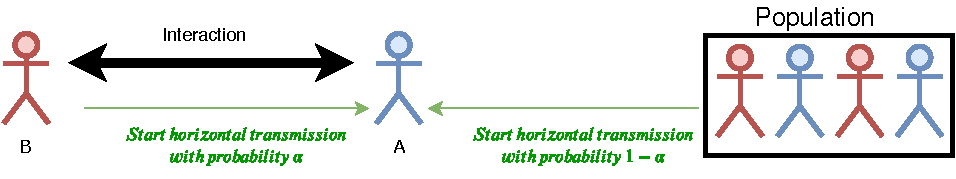
\includegraphics[scale=1]{figure1.pdf}
  \caption{\textbf{Cultural horizontal transmission with assortment.} Transmission occurs between interacting partners with probability $\alpha$ (left) or between two random peers with probability $1-\alpha$, where $\alpha$ is the \emph{social association} parameter.
  }
  \label{fig:horizontal}
\end{figure}



%%% Figure: coexistence map - without oblique transmission
\begin{figure}[htb]
\centering
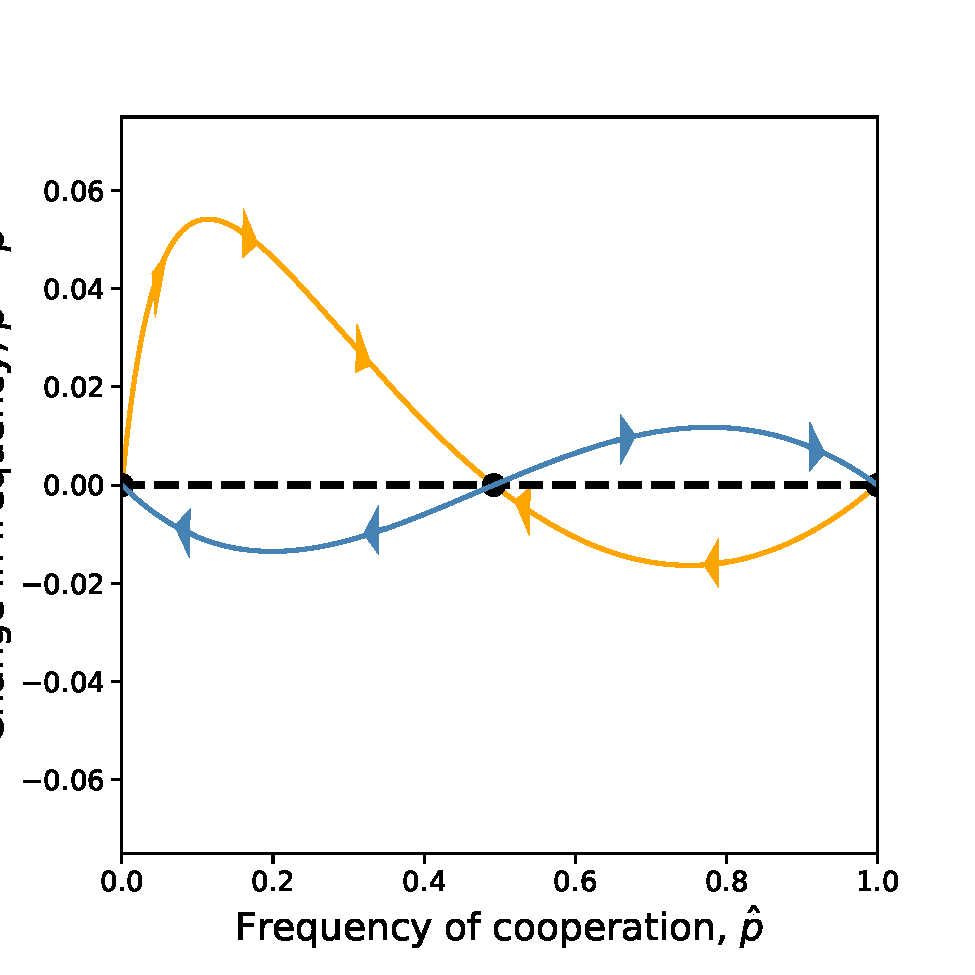
\includegraphics[scale = 0.75]{coexistence_without_oblique.pdf}
\caption{\textbf{Stable and unstable coexistence between cooperation and defection without oblique transmission.}
  The curves show the frequency of the cooperative phenotype $A$ among parents in the next generation, $\tilde{p}'$, vs.\ that in the current generation $\tilde{p}$ (\autoref{eq:nextgen_parents_vertical_only}).
  The dashed black line is $\tilde{p}'=\tilde{p}$.
  The curves and the dashed line intersect at the polymorphic equilibrium $\tilde{p}^*$ (black circle).
  When the curves are above the dashed line, $\tilde{p}'>\tilde{p}$, and $\tilde{p}$ increases.
  When the curves are below the dashed line, $\tilde{p}'<\tilde{p}$, and $\tilde{p}$ decreases.
  The orange curve, for which the polymorphic equilibrium is stable, is given by $T_A = 0.4$, $T_B = 0.9$, $b = 12$, $c=0.35$, and $\alpha = 0.45$, which give $\gamma_2<c<\gamma_1$ (\autoref{eq:cost_boundaries})
  The blue curve, for which the equilibrium is unstable, is given by $T_A = 0.5$, $T_B = 0.1$, $b = 1.3$, $c=0.904$, and $\alpha = 0.4$, which give $\gamma_1<c<\gamma_2$.
  In both cases there is no oblique transmission, $v=1$; see \autoref{fig:coexistence_with_oblique} for $v<1$.
  }
\label{fig:coexistence_without_oblique}
\end{figure}

\pagebreak

%%% Figure: Boundaries figure - only vertical

\begin{figure}[htb]
  \centering       
    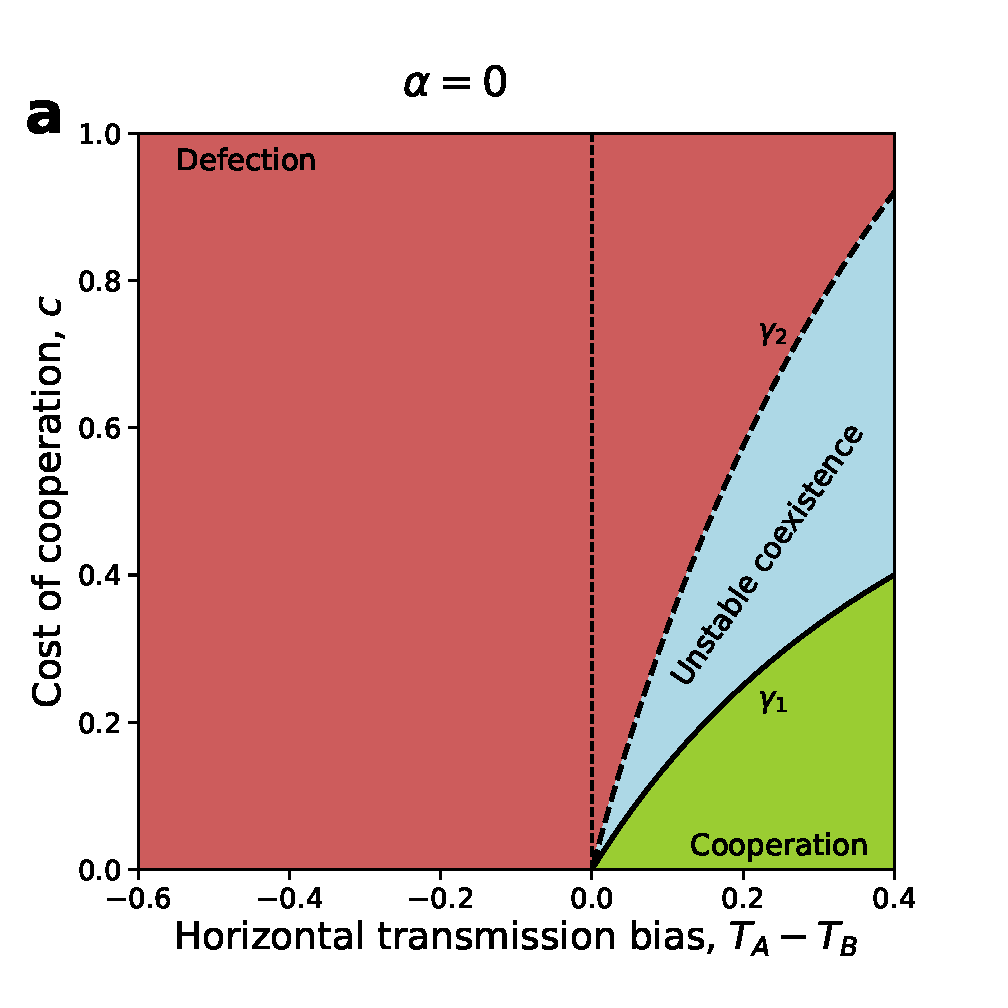
\includegraphics[width=0.45\textwidth]{Result2_c_zero_alpha.eps}
	~
    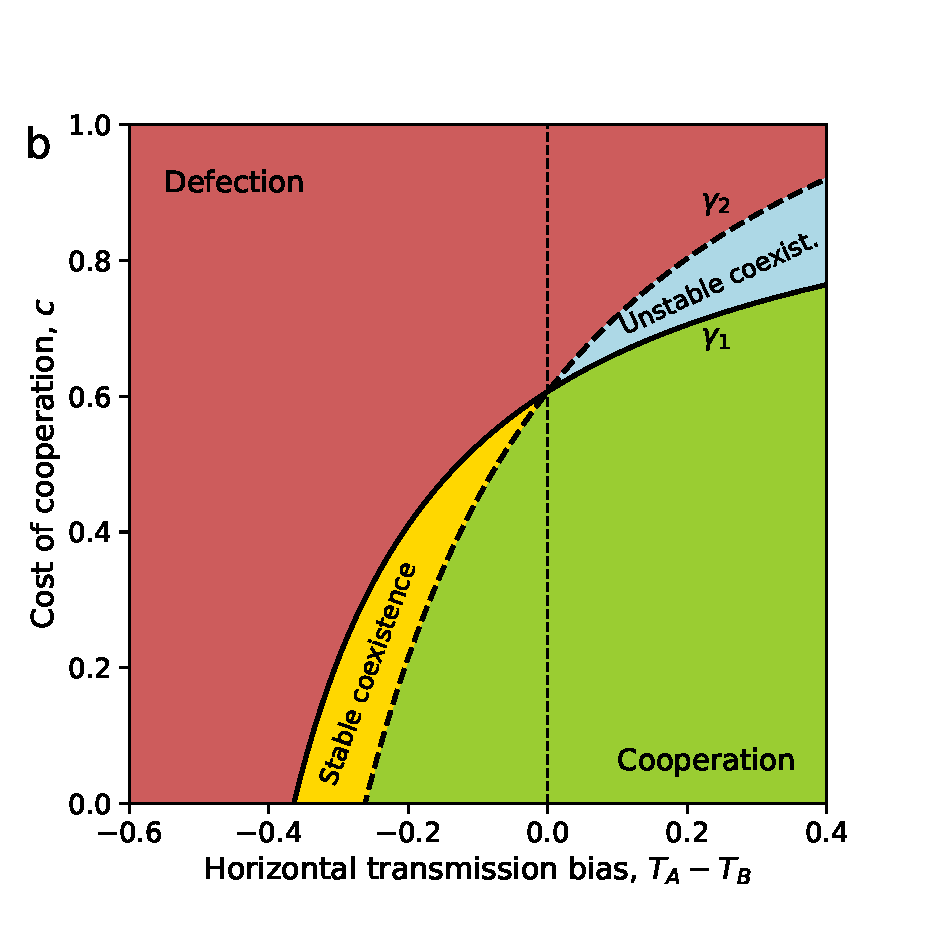
\includegraphics[width=0.45\textwidth]{Result2_c_non_zero_alpha.eps}
    ~
    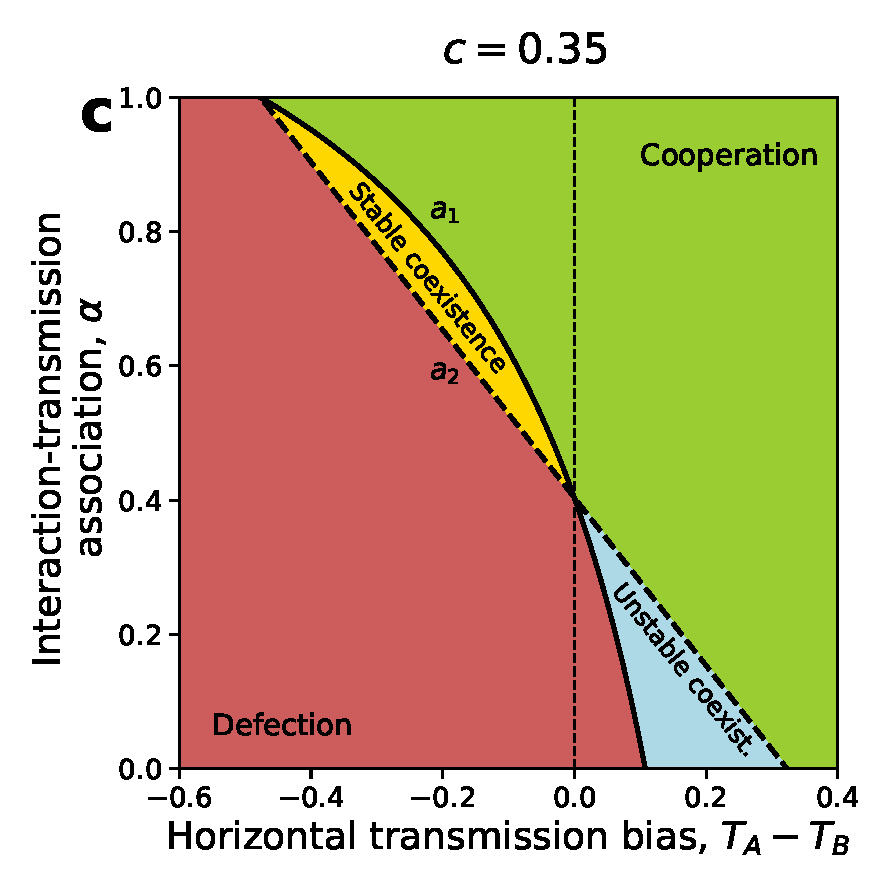
\includegraphics[width=0.45\textwidth]{Result2_alpha.eps}

    \caption{\textbf{Evolution of cooperation under vertical and horizontal cultural transmission.} 
The figure shows the global fixation of cooperation (green), global fixation of defection (red), fixation of either cooperation or defection depending on the initial conditions, i.e. unstable coexistence (blue), and stable coexistence of cooperation and defection (yellow).
In all cases the horizontal bias ($T_A-T_B$) is on the x-axis.
(\textbf{a-b})~The cost of cooperation $c$ is on the y-axis; the cost boundaries $\gamma_1$ and $\gamma_2$ (\autoref{eq:cost_boundaries}) are the solid and dashed lines, respectively. 
(\textbf{c})~social association $\alpha$ is on the y-axis; the social association boundaries $a_1$ and $a_2$ (\autoref{eq:boundries_assortative_meeting}) are the solid and dashed lines, respectively.
Here, $b=1.3$, $T_A=0.4$. (\textbf{a})~$\alpha = 0$.(\textbf{b})~$\alpha = 0.7$. (\textbf{c})~$c = 0.35$.
  	}
    \label{fig:results2}
\end{figure}
\pagebreak

%%% Figure: Boundaries figure - vertical and oblique

\begin{figure}[htb]
  \centering       
    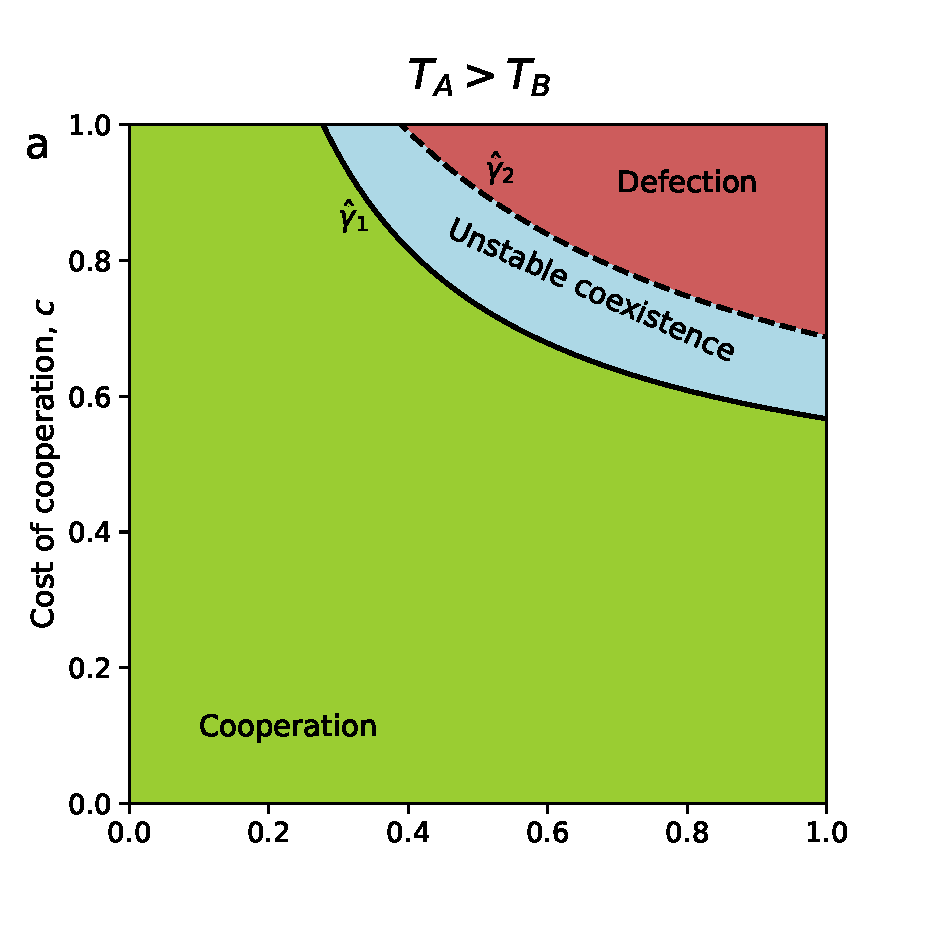
\includegraphics[width=0.45\textwidth]{Result3_TA_TB.eps}~
    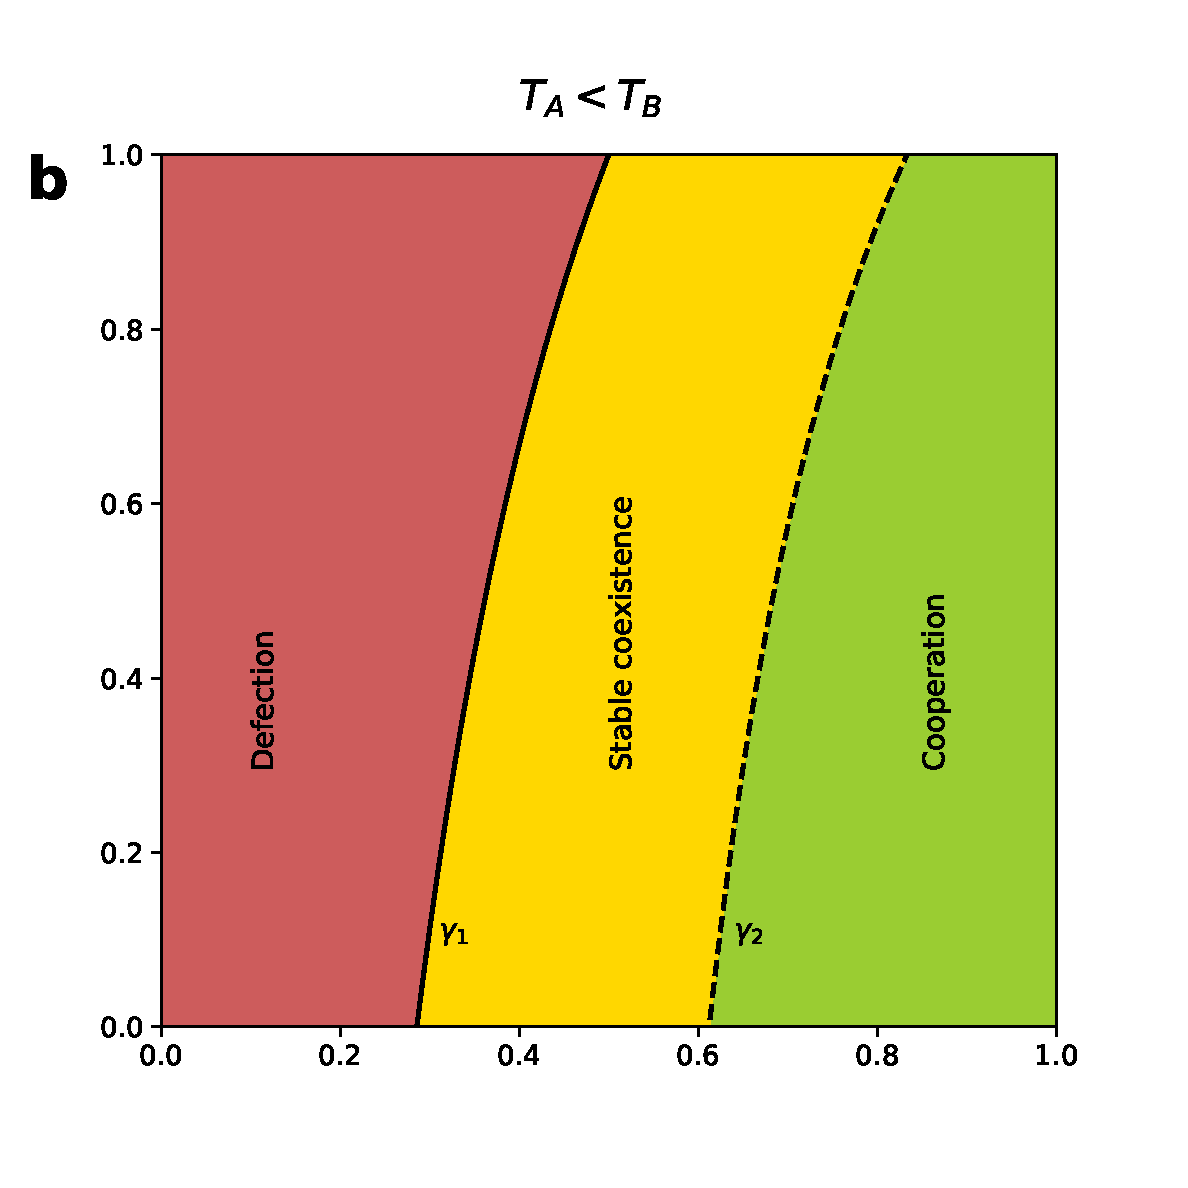
\includegraphics[width=0.45\textwidth]{Result3_TB_TA.eps}
    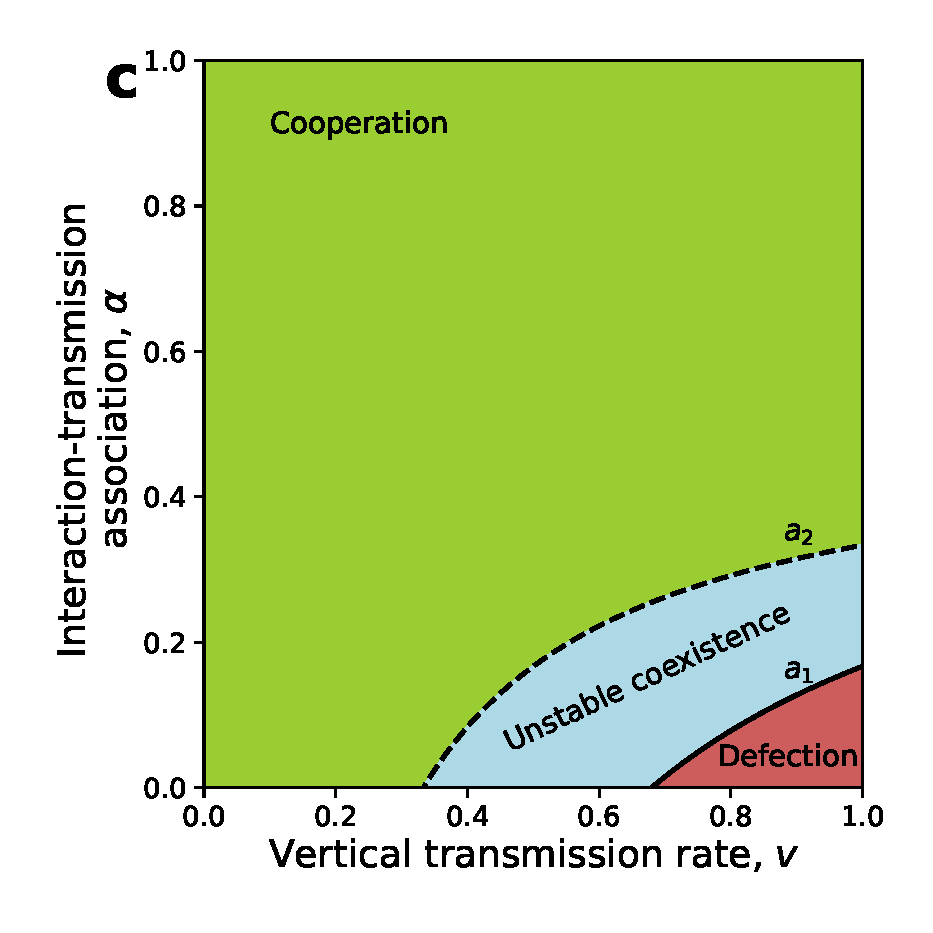
\includegraphics[width=0.45\textwidth]{Result3_alpha_Vs_v_TA_TB.eps}~
    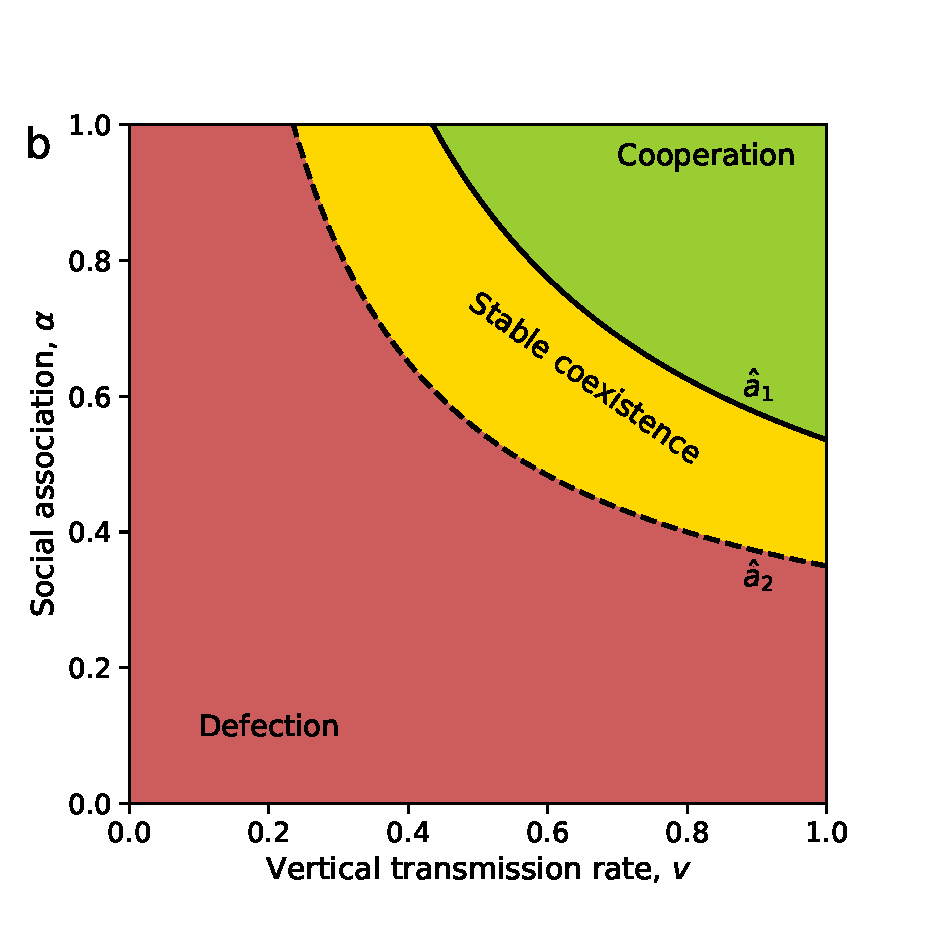
\includegraphics[width=0.45\textwidth]{Result3_alpha_Vs_v_TB_TA.eps}
    \caption{\textbf{Evolution of cooperation under vertical, oblique, and horizontal cultural transmission.} 
    The figure shows the global fixation of cooperation (green), global fixation of defection (red), fixation of either cooperation or defection depending on the initial conditions, i.e. unstable coexistence (blue), and stable coexistence of cooperation and defection (yellow).
	In all cases the vertical transmission rate $v$ is on the x-axis.
	(\textbf{a-b}) The cost of cooperation $c$ is on the y-axis and the cost boundaries $\hat\gamma_1$ and $\hat\gamma_2$ (\autoref{eq:cost_boundaries_v}) are represented by the solid and dashed lines, respectively. 
    (\textbf{c-d}) The social association $\alpha$ is on the y-axis and the social association boundaries $\hat{a}_1$ and $\hat{a}_2$ (\autoref{eq:boundries_assortative_meeting_general_case}) are represented by the solid and dashed lines, respectively. 
    Horizontal transmission is biased in (\textbf{a,c}) for cooperation, $T_A>T_B$, and in (\textbf{b,d}) for defection, $T_A<T_B$.    
    Here, $T_A = 0.5$, and
    (\textbf{a}) $b=1.2$, , $T_B = 0.4$, $\alpha = 0.4$;
    (\textbf{b}) $b=2$, $T_B = 0.7$, $\alpha = 0.7$;
    (\textbf{c}) $b=1.2$, $T_B = 0.4$, $c=0.5$;
    (\textbf{d}) $b=2$, $T_B = 0.7$, $c=0.5$.
    }
    \label{fig:result3}
\end{figure}
\pagebreak

%%% Figure: coexistence map - with oblique transmission
\begin{figure}[htb]
  \centering
  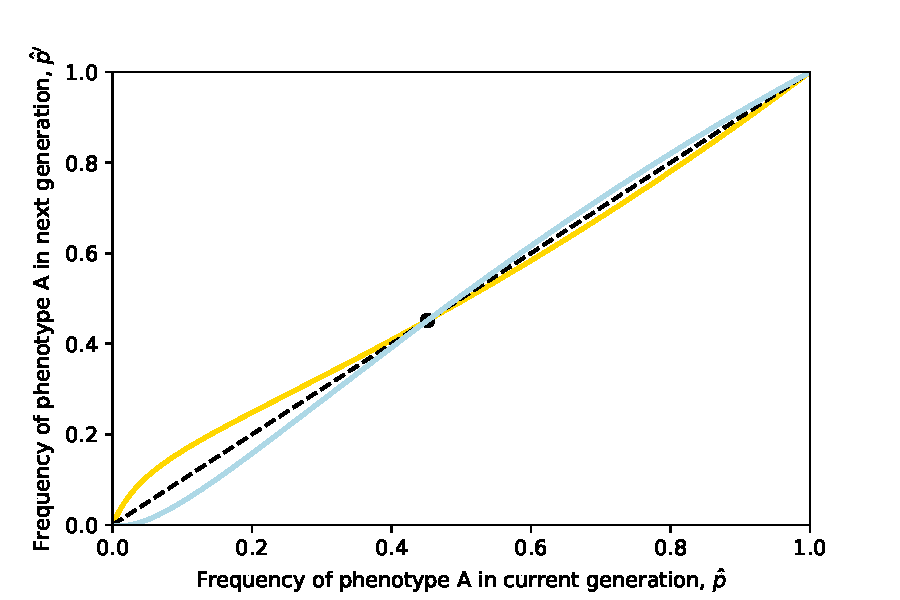
\includegraphics{coexistence_with_oblique.pdf}
  \caption{\textbf{Stable and unstable coexistence between cooperation and defection with oblique transmission.}
  The curves show the frequency $\hat{p}'$ of the cooperative phenotype $A$ among juveniles in the next generation vs. that in current generation $\hat{p}$ (\autoref{eq:horizontal}).
  The dashed black line is $\hat{p}'=\hat{p}$.
  The curves and the dashed line intersect at the stable equilibrium $\hat{p}^*$ (black circle).
  When $\hat{p} < \hat{p}^*$ the curve is above the dashed line, $\hat{p}' > \hat{p}$, and $\hat{p}$ increases towards $\hat{p}^*$.
  When $\hat{p} > \hat{p}^*$ the curve is below the dashed line, $\hat{p}' < \hat{p}$, and $\hat{p}$ decreases towards $\hat{p}^*$.
  The orange curve is parameterized by $T_A = 0.4$, $T_B = 0.9$, $b = 20$, $c=0.1$, $\alpha = 1$, and $v=0.4$, which give $0<\beta_3<\beta_1$ (\autoref{eq:polynomial_coefficients}).
  The blue curve is parameterized by $T_A = 0.5$, $T_B = 0.4$, $b=1.2$, $c=0.487$, $alpha = 0.09$ and $v=0.6$, which give $\beta_1<\beta_3<0$.
  }
  \label{fig:coexistence_with_oblique}
  \end{figure}
\pagebreak

%%% Figure: frequency dynamics
\begin{figure}[htb]
  \centering
    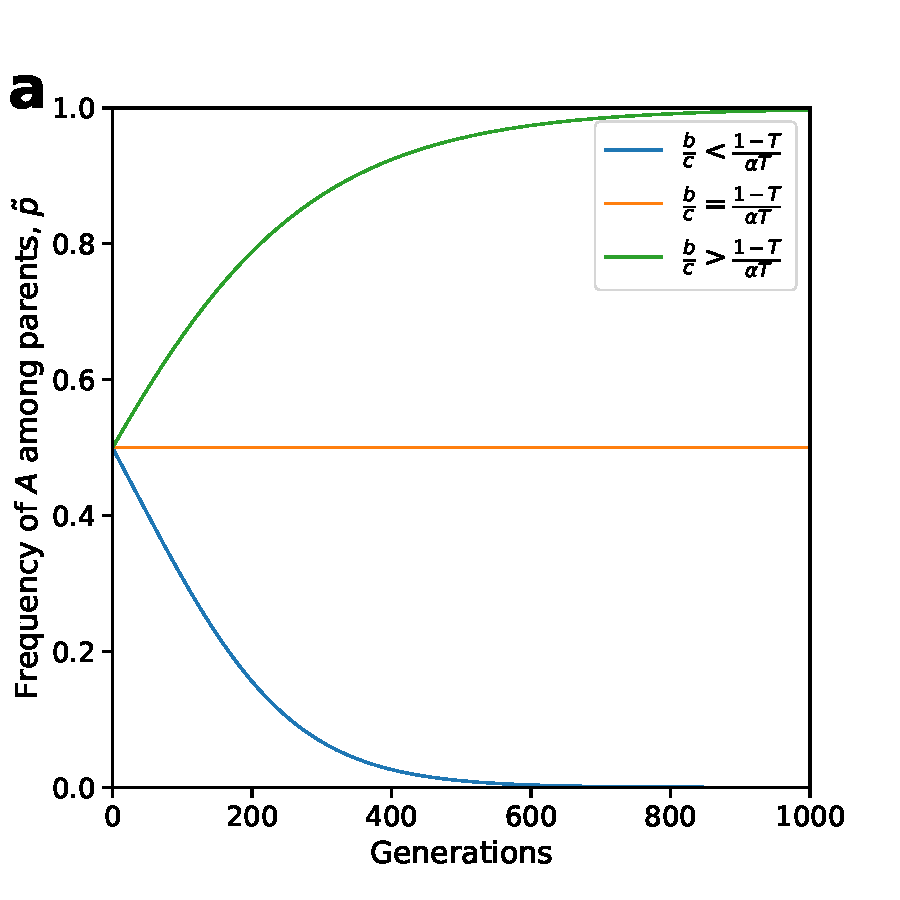
\includegraphics[scale=0.7]{Time_Figure_Equal_Horizontal.pdf}
    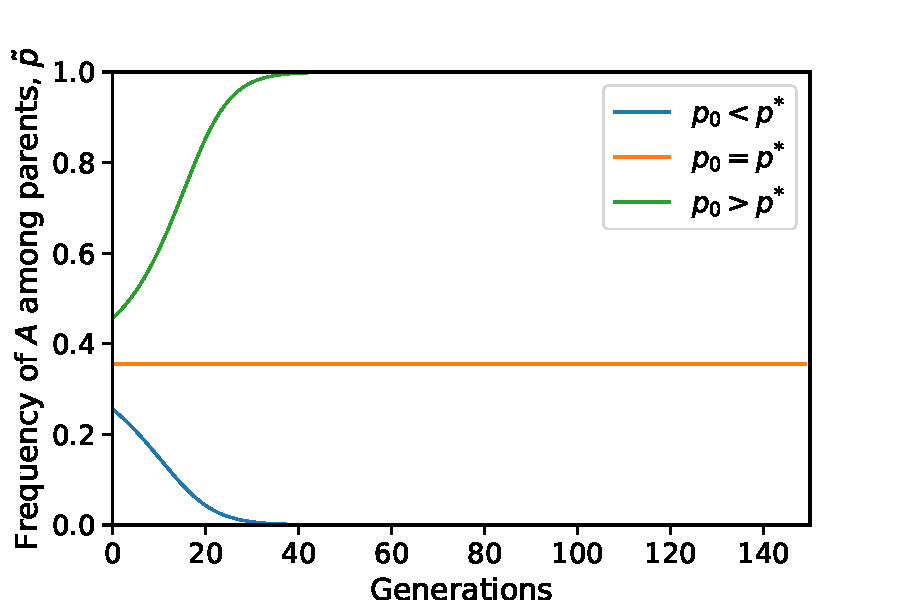
\includegraphics[scale=0.7]{Time_Figure_Only_Vertical_No_Alpha.pdf}
    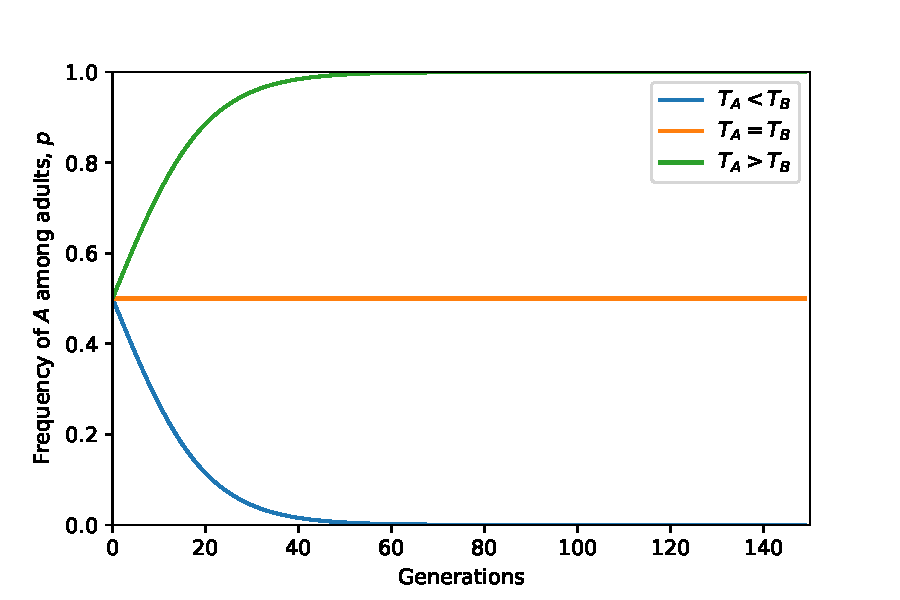
\includegraphics[scale=0.7]{Time_Figure_No_Vertical.pdf}
  \caption{
  \textbf{Dynamics of the frequency of cooperation.}
  The frequency $\tilde{p}$ of parents with cooperative phenotype $A$ in \textbf{(a-b)} and the frequency $p$ of adults with cooperative phenotype $A$ in \textbf{(c)}.
  The different lines correspond to parameter values that lead to fixation of cooperation (green), extinction of cooperation (red), or stable coexistence of cooperators and defectors (yellow).
  \textbf{(a)} $v=1$, $T_A=T_B=T = 0.2$, $\alpha = 0.5 \neq 0$, $\tilde{p}_0 = 0.5$ and $c=0.1$; \textbf{(b)} $v=1$, $\alpha = 0$, $\tilde{p}^* \approx 0.35$, $T_A = 0.65$, $T_B = 0.1$, $b=1.3$ and $c=0.65$; \textbf{(c)} $v=0$, $\alpha =0.5$, $p_0 = 0.5$, $T_A = 0.5$, $b=1.3$ and $c = 0.5$.
  }
  \label{fig:results}
\end{figure}
\pagebreak

%%% Figure: Spatial model
\begin{figure}[htb]
  \centering
    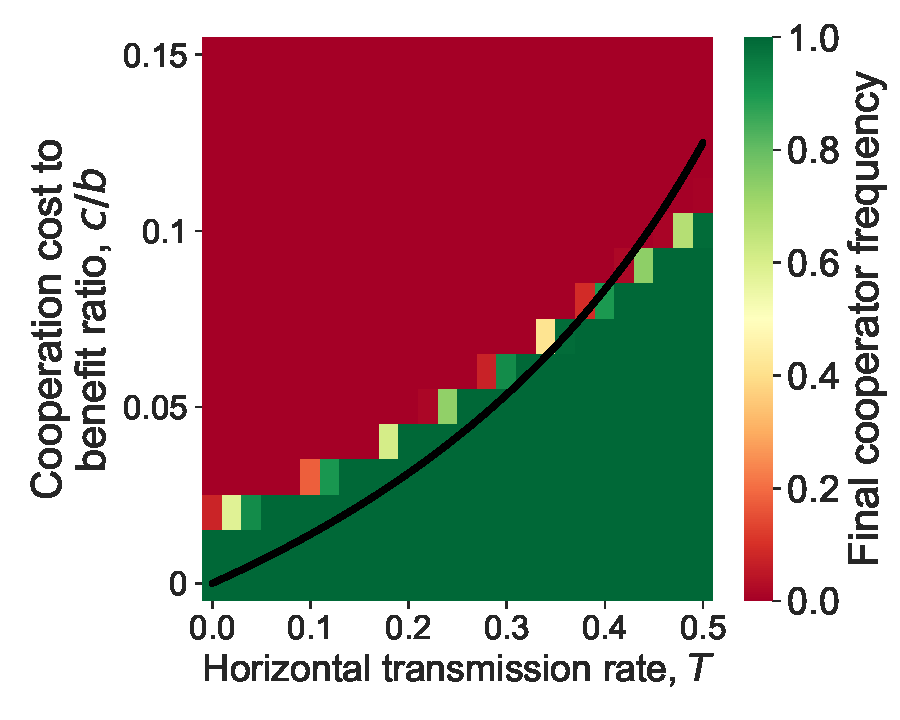
\includegraphics[scale=0.7]{spatial.pdf}
  \caption{
  \textbf{Evolution of cooperation in a spatial model.}
  The expected frequency of cooperators in a structured population after 10,000 generations is shown (red for 0\%, green for 100\%) as function of both the ratio between the cost and benefit of cooperation ($c/b$) on the y-axis, and the horizontal transmission rate (without transmission bias, $T=T_A=T_B$) on the x-axis.
  The population evolves on a 100-by-100 grid. Selection, cooperation, and horizontal cultural transmission are all local between adjacent sites.
  The black curve represents the condition for the evolution of cooperation in a well-mixed population with social association, $c/b<\alpha T / (1-T)$, where $\alpha=1/8$; see \autoref{eq:equal_transmission}.
  Note that in the structured population, selection is local, whereas in the unstructured population, selection is global. This can explain the small difference in the results.
  Here, population size is $10,000$ (100-by-100 grid); cost of cooperation, $c=0.05$. 50 simulations were executed for each parameter set. Simulations were stopped at generation 10,000 or if one of the phenotypes fixed.
  }
  \label{fig:spatial}
\end{figure}

%%%
\end{document}